Improved text about adversarial examples\documentclass[oneside]{book}
%\documentclass[twocolumn]{article}
\usepackage[utf8]{inputenc}
% font
\usepackage{lmodern}
\renewcommand{\familydefault}{\sfdefault}  % sans-serif main

%\usepackage[cm]{sfmath}  % bolje nego mathastext
%\SetSymbolFont{largesymbols}{normal}{OMX}{iwona}{m}{n}

%\usepackage[italic]{mathastext}  % sfmath je bolje (manji indeksi)

%\usepackage{inconsolata}					% sans-serif monospace
\usepackage[scaled]{beramono}				% sans-serif monospace


%\usepackage[math]{iwona}
%\usepackage[math]{kurier}

%\newcommand*{\scale}[2][4]{\scalebox{#1}{$#2$}} % \Scale[0.5]{y = \sin^2 x}
%\usepackage{scalerel}

\usepackage[T1]{fontenc}  % accented characters, copy from pdf, ...

% theorem, definition
\usepackage[english]{babel}
\newtheorem{theorem}{Theorem}
\newtheorem{definition}{Definition}


\raggedright	% no right alignment
\raggedbottom   % no vertical stretching

% Captions
\usepackage{caption}
\captionsetup{%
	justification=raggedright,
}

\usepackage{etoolbox}
\makeatletter
	\patchcmd{\@dottedtocline}
	{\rightskip\@tocrmarg}
	{\rightskip\@tocrmarg plus 4em \hyphenpenalty\@M}
	{}{}
\makeatother
\setlength{\parindent}{1em}	 % uvlačenje ulomaka
\usepackage{indentfirst}	 % uvlačenje prvog ulomka
\setlength{\parskip}{0.5em}	 % razmak između ulomaka

\usepackage{listings}  % listings
\renewcommand{\lstlistingname}{Ispis}

\usepackage[multiple, bottom]{footmisc}	 % višestruke fusnote, poslije slika/tablica

\usepackage[hidelinks]{hyperref}
\renewcommand*{\UrlFont}{\footnotesize}

% colors

\usepackage{xcolor}
\usepackage{color}

\hypersetup{
	colorlinks,
	linkcolor={blue!60!green!50!black},  % xcolor package
	citecolor={green!40!black},
	urlcolor={blue!75!green!30!black}
}
\definecolor{bluekeywords}{rgb}{0.13,0.13,1}  % color package
\definecolor{greencomments}{rgb}{0,0.5,0}
\definecolor{redstrings}{rgb}{0.9,0,0}

%\newtheorem{theorem}{Teorem}[section]
%\newtheorem{definition}{Definicija}[section]

\usepackage{enumitem} \setlist[enumerate,1]{topsep=0pt,itemsep=0pt,partopsep=0pt}
\setlist[itemize,1]{topsep=0pt,itemsep=0pt,partopsep=0pt}

 
\DeclareTextFontCommand{\emphasize}{\bfseries}

\newcommand{\say}[1]{"\textit{#1}}

% redefinition of left and right to make spacing consistent
\let\originalleft\left
\let\originalright\right
\def\left#1{\mathopen{}\originalleft#1}
\def\right#1{\originalright#1\mathclose{}}

\usepackage{amsmath}
\usepackage{amssymb}  % loads amsfonts

\usepackage{mathtools}  % \coloneqq
%\usepackage{bm}
%\usepackage[utopia]{mathdesign}
\usepackage[OMLmathsfit]{isomath}  % \DeclareMathAlphabet ...

\usepackage{mathtools}  % smashoperator
\usepackage{upgreek}

%\usepackage{commath}  % calculus, perentheses
% https://tex.stackexchange.com/questions/135944/commath-and-ifinner/135985#135985
%
\DeclareMathOperator{\dif}{d \!}
\DeclareMathOperator{\Dif}{D \!}

\makeatletter
\newcommand{\spx}[1]{%
	\if\relax\detokenize{#1}\relax
	\expandafter\@gobble
	\else
	\expandafter\@firstofone
	\fi
	{^{#1}}%
}
\makeatother

\newcommand\pd[3][]{\frac{\partial\spx{#1}#2}{\partial#3\spx{#1}}}
\newcommand\tpd[3][]{\tfrac{\partial\spx{#1}#2}{\partial#3\spx{#1}}}
\newcommand\dpd[3][]{\dfrac{\partial\spx{#1}#2}{\partial#3\spx{#1}}}

\newcommand{\md}[6]{\frac{\partial\spx{#2}#1}{\partial#3\spx{#4}\partial#5\spx{#6}}}
\newcommand{\tmd}[6]{\tfrac{\partial\spx{#2}#1}{\partial#3\spx{#4}\partial#5\spx{#6}}}
\newcommand{\dmd}[6]{\dfrac{\partial\spx{#2}#1}{\partial#3\spx{#4}\partial#5\spx{#6}}}

\newcommand{\od}[3][]{\frac{\dif\spx{#1}#2}{\dif#3\spx{#1}}}
\newcommand{\tod}[3][]{\tfrac{\dif\spx{#1}#2}{\dif#3\spx{#1}}}
\newcommand{\dod}[3][]{\dfrac{\dif\spx{#1}#2}{\dif#3\spx{#1}}}

\newcommand{\genericdel}[4]{%
	\ifcase#3\relax
	\ifx#1.\else#1\fi#4\ifx#2.\else#2\fi\or
	\bigl#1#4\bigr#2\or
	\Bigl#1#4\Bigr#2\or
	\biggl#1#4\biggr#2\or
	\Biggl#1#4\Biggr#2\else
	\left#1#4\right#2\fi
}
\newcommand{\del}[2][-1]{\genericdel(){#1}{#2}}
\newcommand{\set}[2][-1]{\genericdel\{\}{#1}{#2}}
\let\cbr\set
\let\event\set
\newcommand{\sbr}[2][-1]{\genericdel[]{#1}{#2}}
\let\intoo\del
\let\intcc\sbr
\newcommand{\intoc}[2][-1]{\genericdel(]{#1}{#2}}
\newcommand{\intco}[2][-1]{\genericdel[){#1}{#2}}
\newcommand{\eval}[2][-1]{\genericdel.|{#1}{#2}}
\newcommand{\envert}[2][-1]{\genericdel||{#1}{#2}}
\let\abs\envert
\newcommand{\sVert}[1][0]{%
	\ifcase#1\relax
	\rvert\or\bigr|\or\Bigr|\or\biggr|\or\Biggr
	\fi
}
\newcommand{\enVert}[2][-1]{\genericdel\|\|{#1}{#2}}
\let\norm\enVert
\newcommand{\fullfunction}[5]{%
	\begin{array}{@{}r@{}l@{}}
		#1 \colon #2 &{}\longrightarrow{}  #3 \\
		#4 &{}\longmapsto{} #5
	\end{array}
}
%
%


\usepackage{stmaryrd}  % \llbracket for \rrbracket, ...


%\usepackage[croatian]{babel}		% teorem
%\newtheorem{definition}{Definicija}[section]
%\newtheorem{theorem}{Teorem}[section]
%\newtheorem{corollary}{Korolar}[theorem]

\DeclareMathAlphabet{\mathbbmsl}{U}{bbm}{m}{sl}
\DeclareMathAlphabet{\mathbbmb}{U}{bbm}{b}{it}
\DeclareMathAlphabet{\mathbbmssit}{U}{bbmss}{m}{it}


% common set?, distribution
\newcommand{\commset}[1]{\mathbbmb{#1}}
\newcommand{\distrib}[1]{\mathcal{#1}}

% sans-serif blackboard-bold
\newcommand{\mathsfbbit}[1]{\mathbbmssit{#1}}

% variable
\let\vec\relax
\let\set\relax
\newcommand{\vec}[1]{\mathbfit{#1}}
\newcommand{\set}[1]{\mathbbmsl{#1}}

% constant
\newcommand{\const}[1]{\mathrm{#1}}
\newcommand{\cvec}[1]{\mathbf{#1}}
\newcommand{\cset}[1]{\mathbb{#1}}

% random variable
%\newcommand\mathmakebox[3][1em][c]{\mathpalette\mathmakeboxinternal[#1][#2]{#3}}
%\newcommand\mathmakeboxinternal[3][1em][c]{\makebox[#1][#2]{$\mathsurround=0pt{#3}$}}
\usepackage{etex}
\newcommand{\nunder}[2][5]{\mathrlap{\mkern\the\numexpr#1/2mu\relax\underline{\phantom{\mathrm{#2}\mkern-#1mu}}}\mathrm{#2}}
\newcommand{\subline}[2][n]{%
    \makebox[\widthof{$#2$}/2]{}\mathclap{#2}%
    \text{\smash{\raisebox{0.04em}{% 0.04
        $\mathclap{\underline{\hphantom{#1}\vphantom{#2}}}$%
    }}}%
    \makebox[\widthof{$#2$}/2]{}%
}
\newcommand{\rvarstyle}[1]{{{\subline[i]{#1}}}}
\newcommand{\rvar}[1]{\rvarstyle{#1}}
\newcommand{\rvec}[1]{\rvarstyle{\vec{#1}}}
\newcommand{\rset}[1]{\rvarstyle{\set{#1}}}
\newcommand{\var}[1]{{\color{red}#1}}

% linear algebra
\newcommand{\transpose}{\mathsf T}
\newcommand{\tp}{\transpose}

% calculus - commath: od, pd, md, dif
% parentheses - commath: del, cbr, sbr, envert, enVert

% named functions
\DeclareMathOperator{\softplus}{softplus}
\DeclareMathOperator{\softmax}{softmax}
\DeclareMathOperator{\logistic}{\sigma}
\DeclareMathOperator{\sgn}{sgn}
\DeclareMathOperator{\diag}{diag}
\DeclareMathOperator{\ReLU}{ReLU}
\DeclareMathOperator{\modfunc}{mod}

% operators
\DeclareMathOperator*{\argmin}{arg\,min} % thin space
\DeclareMathOperator*{\argmax}{arg\,max}
\let\P\relax
\newcommand{\P}{\mathrm{P}}
\newcommand{\p}{\mathrm{p}}
\DeclareMathOperator*{\E}{\mathrm{I\kern-.282em E}}
\DeclareMathOperator*{\D}{\mathrm{I\kern-.282em D}}
\DeclareMathOperator*{\Cov}{\mathrm{Cov}}
%\let\H\relax
\renewcommand{\H}{\mathrm{H}}
\newcommand{\h}{\mathrm{h}}
\newcommand{\I}{\mathrm{I}}
\newcommand{\Dist}{\mathrm{D}}  % D is for dispersion
%\renewcommand{\dif}{\mathrm{d}}

\newcommand{\pa}{\mathrm{pa}}
\newcommand{\ch}{\mathrm{ch}}
\newcommand{\pred}{\mathrm{pred}}
\renewcommand{\succ}{\mathrm{succ}}

\newcommand{\vecfunc}{\mathrm{vec}}

% bracket operators
%\newcommand{\enangle}[1]{\mathinner{\left\langle{#1}\right\rangle}}
\newcommand{\enangle}[2][-1]{\genericdel\langle\rangle{#1}{#2}}
\newcommand{\enbbracket}[1]{{\mathinner{\left\llbracket{#1}\right\rrbracket}}}
\newcommand{\braket}[2]{\enangle{{#1}\middle|{#2}}}

% parentheses from commath redefined to improve spacing because left and right were redefined, \midmid, new \tilde and \hat that don't make parentheses bigger
\renewcommand{\del}[1]{\left(#1\right)}
\renewcommand{\sbr}[1]{\left[#1\right]}
\renewcommand{\cbr}[1]{\left\{#1\right\}}
\renewcommand{\intoo}[1]{\mathinner{\del{#1}}}
\renewcommand{\intcc}[1]{\mathinner{\sbr{#1}}}
\renewcommand{\intco}[1]{\mathinner{\left[#1\right)}}
\renewcommand{\intoc}[1]{\mathinner{\left(#1\right]}}
\newcommand{\ind}[1]{{\sbr{#1}}}
%\let\mid\relax
%\newcommand{\mid}{\;|\;}  % spaces around not reduced in index
\newcommand{\midmid}{\;\middle|\;}
\let\oldhat\hat
\renewcommand{\hat}[1]{\vphantom{#1}\smash[t]{\oldhat{#1}}}
\let\oldtilde\tilde
\renewcommand{\tilde}[1]{\vphantom{#1}\smash[t]{\oldtilde{#1}}}
%\renewcommand{\tilde}[1]{\stackrel{\sim}{\smash{\mathcal{#1}}\rule{0pt}{1.1ex}}}
%\renewcommand{\tilde}[1]{\overset{\sim}{#1}}}
\let\oldwidetilde\widetilde
\renewcommand{\widetilde}[1]{\vphantom{#1}\smash[t]{\oldwidetilde{#1}}}

% special
%\newcommand{\funcdef}[3]{#1 \in (#2 \to #3)}
\newcommand{\funcdef}[3]{#1 \colon #2 \to #3}
\newcommand{\Dkl}[2]{\Dist_\mathrm{KL}\del{#1\;\middle\|\;#2}}
\newcommand{\C}{\cset{C}}
\newcommand{\R}{\cset{R}}
\newcommand{\Z}{\cset{Z}}
\newcommand{\N}{\cset{N}}
\newcommand{\dirac}{\updelta}

\newcommand\concat{\mathbin{+\mkern-10mu+}}

\newcommand{\TP}{\mathit{TP}}
\newcommand{\FP}{\mathit{FP}}
\newcommand{\TN}{\mathit{TN}}
\newcommand{\FN}{\mathit{FN}}
\newcommand{\FPR}{\mathit{FPR}}
\newcommand{\TPR}{\mathit{TPR}}
\newcommand{\AUROC}{\mathit{AUROC}}
\newcommand{\AUPR}{\mathit{AUPR}}
\newcommand{\AP}{\mathit{AP}}
\newcommand{\IoU}{\mathit{IoU}}
\newcommand{\mIoU}{\mathit{mIoU}}

% operators and relations
\newcommand{\bidot}{\mkern1.5mu{..}\mkern1.5mu}
%\newcommand\sheq{\mkern1.5mu{=}\mkern1.5mu}
%\renewcommand{\dots}{...}


% no vertical space stretching around display math
\usepackage[nodisplayskipstretch]{setspace}

\newenvironment{talign}
{\let\displaystyle\textstyle\align}
{\endalign}
\newenvironment{talign*}
{\let\displaystyle\textstyle\csname align*\endcsname}
{\endalign}


\usepackage{dashbox}%
%\newcommand\dashedbox[1][H]{\setlength{\fboxsep}{0pt}\setlength{\dashlength}{4pt}\setlength{\dashdash}{2pt} \dbox{\phantom{#1}}}
\newcommand\phbox[1][\phantom{:}]{\setlength{\fboxsep}{0.5pt}\setlength{\dashlength}{4pt}\setlength{\dashdash}{3pt} \raisebox{2pt}{\dbox{$\phantom{:}_{#1}$}}}
%\newcommand\dashedbox[1][H]{\setlength{\fboxsep}{0pt}\dbox{\phantom{#1}}}

\usepackage{booktabs}  % from the tamplate; table quality enhancement

\usepackage{multirow}
\usepackage{tabularx}
\usepackage{tabu}
\usepackage{makecell}

\newcolumntype{P}[1]{>{\raggedright\let\newline\\\arraybackslash\hspace{0pt}}p{#1}}

\renewcommand{\arraystretch}{1.1}
%\usepackage{floatrow} 				% centriranje svih slika
\usepackage{float}					% figure [H]
\usepackage{graphicx} 				% includegraphics
\usepackage{caption}			% subfigure
\usepackage{subcaption}			% subfigure
\usepackage[export]{adjustbox} 	% http://ctan.org/pkg/adjustbox

\usepackage[section]{placeins}  % [section] for \FloatBarrier before every section 

\graphicspath{ {./figures/} }		% mapa sa slikama
%\let\oldincludegraphics\includegraphics
%\renewcommand{\includegraphics}[2][]{\oldincludegraphics[#1,max width=0.9\linewidth]{#2}}

%\usepackage{flafter} % floats after the first reference

\usepackage{tikz} 					% dijagrami
\usepackage{pgfplots}
\usetikzlibrary{fit,automata,arrows,positioning,calc,petri,topaths,arrows.meta}

%\usetikzlibrary{external}
%\tikzexternalize[prefix=figures/tikz/, shell escape=-enable-write18]
%TexStudio Configuration\commands\pdflatex:
%"pdflatex.exe -src -interaction=nonstopmode --shell-escape %.tex

\pgfplotsset{every axis/.append style={
		axis x line=middle,    	% put the x axis in the middle
		axis y line=middle,    	% put the y axis in the middle
		axis line style={->},  	% arrows on the axis
		xlabel={$x$},          	% default put x on x-axis
		ylabel={$y$},          	% default put y on y-axis
		samples=100,
		axis equal,
}} % axis style

\tikzset{
	>={Triangle[length=1.8mm,width=1.2mm]},
	dedge/.style={arrows=->, black, thick},
}
% PGMs
\tikzstyle{textnode} = [minimum size=5mm, node distance=9mm]
\tikzstyle{pnode} = [circle, minimum size=10mm, thick, draw=black, node distance=9mm]
\tikzstyle{greypnode} = [pnode, fill=black!5]
% https://github.com/jluttine/tikz-bayesnet
\tikzstyle{wrap} = [inner sep=0pt, fit=#1]
\tikzstyle{plate} = [draw, rectangle, rounded corners=0.5ex, thick, fit=#1]
\tikzstyle{caption} = [font=\footnotesize, node distance=0]
\tikzstyle{plate caption} = [caption, node distance=0, inner sep=0pt,
below left=5pt and 0pt of #1.south east]
\newcommand{\plate}[4][]{
	\node[wrap=#3] (#2-wrap) {};
	\node[plate caption=#2-wrap] (#2-caption) {#4};
	\node[plate=(#2-wrap)(#2-caption), #1] (#2) {};
}
% ANNs
\tikzstyle{nnode} = [circle, minimum size=10mm, thick, draw=black, node distance=5mm]
\tikzstyle{nrect} = [rectangle, minimum size=7mm, thick, draw=black, node distance=5mm, rounded corners=0.1ex]
\usepackage{dirtree}

\usepackage[]{algorithmic}

\usepackage{setspace}  % line spacing

\usepackage{pdfpages} % inclusion of external pdf pages

\usepackage[toc]{appendix}
%\usepackage[sort&compress,round,comma,authoryear]{natbib}
\usepackage{natbib}

\title{Machine learning notes}
\author{}
\date{}

\usepackage[symbols,nopostdot,nonumberlist,section]{glossaries-extra}

%\renewcommand{\glossarypreamble}{\footnotesize}

\newglossarystyle{supergroup}{%
	\setglossarystyle{super}%
	\renewcommand*{\glsgroupskip}{}%
	\renewcommand{\glossentry}[2]{%
		\tabularnewline%
		\multicolumn{2}{p{\textwidth}}{%
			\raggedright\glsentryitem{##1}\glstarget{##1}{\glossentryname{##1}}%
		}% 
		\vspace{2mm}%
		\tabularnewline%
	}%
	\renewcommand{\subglossentry}[3]{%
		\glssubentryitem{##2}%
		\glstarget{##2}{\glossentryname{##2}}&%
		\raggedright\glossentrydesc{##2}\glspostdescription\space##3\tabularnewline%
	}%
}
\newcommand{\test}[1]{ \def\tst{#1} \ifx\tst\empty \typeout{optional argument was omitted} \else \typeout{optional argument was given: '#1'} \fi}
\newcommand{\glsgroup}[3]{%
	\newglossaryentry{#1}{type=symbols, name={{\large \textbf{#2}} \def\temp{#3}\ifx\temp\empty\else\vspace{2mm}\newline #3\fi}, description={}}
}
\newcommand{\glsent}[4]{\newglossaryentry{{#1:#2}}{sort={#2},type=symbols,name={#3},description={#4},parent={#1}}}
\newcommand{\glsentm}[4]{\glsent{#1}{#2}{\ensuremath{\displaystyle#3}}{#4}}

%\setglossarypreamble[symbols]{Ovaj odjeljak sadrži popis velikog broja oznaka koje se koriste u ovom radu. Za neke skupine oznaka napisana su kratka objašnjenja koja dodatno pojašnjavaju i opravdavaju neke oznake. Pojmovi koje označavaju neke oznake detaljnije su objašnjeni u poglavlju~\ref{chap:osnovni-pojmovi}.}

% Objekti
\glsgroup{o}{Objects}
{Variables are generally denoted by italic serif letters. Most constants are denoted by upright serif letters. Random variables are underlined. Vectors and sequences are denoted by lowercase bold letters. Matrices and multidimensional-arrays are denoted by uppercase bold letter. Sets are denoted by uppercase blackboard-bold letters. Latin or Greek letters can be used for any type of object.}
\glsentm{o}{var}{a,\,A,\,\theta}
	{Variable (commonly scalar or function)}
\glsentm{o}{vec}{\vec a,\,\vec\theta}
	{Vector or sequence (commonly column vector)}
\glsentm{o}{mat}{\vec A,\,\vec\Theta}
	{Matrix or multidimensional array}
\glsentm{o}{set}{\set A}
	{Set or multiset}
\glsentm{o}{const}{\const a,\,\const A,\,\uptheta}
	{Constant}
\glsentm{o}{cvec}{\cvec a,\,\boldsymbol{\uptheta}}
	{Vector or sequence constant}
\glsentm{o}{cmat}{\cvec A,\,\cvec\Theta}
	{Matrix or multidimensional array constant}
\glsentm{o}{cset}{\cset A}
	{Set constant}
\glsentm{o}{rvar}{\rvar a,\,\rvar A,\,\rvar\theta}
	{Random variable}
\glsentm{o}{rvec}{\rvec a,\,\rvec\theta}
	{Random vector or sequence}
\glsentm{o}{rmat}{\rvec A,\,\rvec\Theta}
	{Random matrix or multidimensional array}
\glsentm{o}{rset}{\rset A}
	{Random set or multiset}
\glsentm{o}{text}{\text{a},\,\text{riječ}}
	{Textual label not representing an object}

% Konstante
\glsgroup{k}{Constants}{}
\glsentm{k}{emptyset}{\cbr{}}
	{Enpty set}
\glsentm{k}{e}{\const e}
	{The number that satisfies $\od{}{x}\const e^x=\const e^x$}
\glsentm{k}{nulvek}{\cvec 0}
	{Null-vector}
\glsentm{k}{kanvek}{\cvec e_i}
	{$i$-th canonical basis vector}
\glsentm{k}{jedvek}{\cvec 1}
	{The sum of all canonical basis vectors}
\glsentm{k}{mati}{\cvec I,\,\cvec I_n}
	{Identity matrix (with $n$ rows/columns)}
\glsentm{k}{cset}{\N,\Z,\R,\C}
	{A standard set}
\glsentm{k}{Rpos}{\R_{\geq 0},\,\R_{> 0}}
	{The set of all non-negative/positive real numbers}

% Skupovi i nizovi
\glsgroup{sn}{Defining sets and arrays}{}
\glsentm{sn}{range}{a\bidot b}
	{Shorthand notation for $a,..,b$}
\glsentm{sn}{setrange}{\cbr{a\bidot b}}
	{A subset of integers from $a$ to $b$}
\glsentm{sn}{setdefset}{\cbr{f(a)\colon P(a)},\, \cbr{f(a)}_{P(a)}}
	{A set with elements defined by a function $f$ and a predicate $P$}
\glsentm{sn}{setdefsetimp}{\cbr{f(a)}_{a}}
	{A set with elements defined by a function $f$ and variables $a$ from an implicitly defined set}
\glsentm{sn}{setdefn}{\cbr{a_1\bidot a_n},\,\cbr{a_i}_{i=1\bidot n}}
	{A set with $n$ elements}
\glsentm{sn}{rowvec}{\sbr{x_1,\bidot,x_n}}
	{A row vector}
\glsentm{sn}{ndarrdef}{\sbr{a_i}_{i}, \sbr{a_{i,j}}_{i,j}, \sbr{a_{i,j,k}}_{i,j,k}}
	{A multidimensional array with an implicit or undefined number of elements}
\glsentm{sn}{intco}{\intco{a,b}}
	{A semi-closed interval}
%\glsentm{sn}{colvec}{\del{x_1,\bidot,x_n}}
%	{$n$-torka}

% Donji i gornji indeks
\glsgroup{i}{Subscript and superscript}
{U donjem i gornjem indeksu oznake mogu biti oznake drugih matematičkih objekata ili slova ili riječi koje ne predstavljaju matematičke objekte. Redni brojevi elemenata vektora ili višedimenzionalnih nizova se, ako nije određeno drugačije, pišu u donjem indeksu oznake vektora u uglatim zagradama. Npr. $i$-ti element vektora $\vec a=\sbr{a_1,.., a_n}^\tp$ je $\vec a_\ind{i}=a_i$. Indeksi kod $n$-dimenzionalnih nizova mogu biti i vektori iz $\N^{n}$, ili kombinacije vektora manje dimenzije sa skalarima.}
\glsentm{i}{gdindeks}{a_\text{d}^\text{g}}
	{Varijabla s oznakama u donjem i gornjem indeksu}
\glsentm{i}{vecelem}{\vec{a}_\ind{i}}
	{$i$-ti element vektora $\vec{a}$}
\glsentm{i}{subvec}{\vec{a}_\ind{i_1:i_2}}
	{Vektor kojeg čine elementi $\vec{a}_\ind{i_1}, \vec{a}_\ind{i_1+1},.., \vec{a}_{\sbr{i_2}}$}
\glsentm{i}{subvecsk}{\vec{a}_\ind{(i_1\bidot i_n)}}
	{Vektor kojeg čine elementi $\vec{a}_\ind{i_1}, \vec{a}_\ind{i_2},.., \vec{a}_{\sbr{i_n}}$}
\glsentm{i}{matelem}{\vec{A}_\ind{i,j}}
	{Element $i,j$ matrice $\vec A$}
\glsentm{i}{matrow}{\vec{A}_\ind{i,:}}
	{$i$-ti redak matrice $\vec A$}
\glsentm{i}{asubmat}{\vec{A}_\ind{:,i_1:i_2,j}}
	{2-D odsječak 3-D niza $\vec A$}
\glsentm{i}{aet}{\vec{A}_\ind{\vec i}}
	{Element $\vec{A}_\ind{\vec i_\ind{1},\bidot,\vec i_\ind{n}}$ $n$-D niza}
\glsentm{i}{ast}{\vec{A}_\ind{\vec i_1:\vec i_2}}
	{Podniz $\vec{A}_\ind{{\vec i_1}_\ind{1}:{\vec i_2}_\ind{1},\bidot,{\vec i_1}_\ind{n}:{\vec i_2}_\ind{n}}$ $n$-D niza}
\glsentm{i}{astp}{\vec{A}_\ind{\vec i_1:\vec i_2;:}}
	{Podniz $\vec{A}_\ind{{\vec i_1}_\ind{1}:{\vec i_2}_\ind{1},\bidot,{\vec i_1}_\ind{n-1}:{\vec i_2}_\ind{n-1},:}$ $n$-D niza}

% Operacije linearne algebre i operacije s nizovima
\glsgroup{l}{Operacije linearne algebre i operacije s nizovima} {} 
\glsentm{l}{scalprod}{\braket{\vec a}{\vec b},\,\vec{a}^\tp\vec{b}}
	{Skalarni produkt}
\glsentm{l}{outprod}{\vec{a}\vec{b}^\tp}
	{Vanjski produkt}
\glsentm{l}{hadprod}{\vec a \odot \vec b}
	{Umnožak po elementima; Hadamardov produkt}
\glsentm{l}{haddiv}{\vec a \oslash \vec b}
	{Dijeljenje po elementima}
\glsentm{l}{hadpow}{\vec a^{\odot b}}
	{Potenciranje po elementima}
\glsentm{l}{matmul}{\vec A \vec B}
	{Matrično množenje}
\glsentm{l}{matinv}{\vec A^{-1}}
	{Inverz matrice}
\glsentm{l}{transp}{\vec A^\tp}
	{Transponiranje}
\glsentm{l}{diag}{\diag\del{\vec{a}}}
	{Dijagonalna matrica kojoj dijagonalu čini vektor $\vec a$}
\glsentm{l}{det}{\det(\vec{A})}
	{Determinanta matrice $\vec A$}
\glsentm{l}{vecl2norm}{\enVert{\vec a}_2}
	{$\const L^2$-norma vektora $\vec a$}
\glsentm{l}{vecnorm}{\enVert{\vec a}_p}
	{$\const L^p$-norma vektora $\vec a$}
\glsentm{l}{matnorm}{\enVert{\vec A}_p}
	{Matrična $\const L^p$-norma matrice $\vec A$}
\glsentm{l}{frobnorm}{\enVert{\vec A}_\text{F}}
	{Frobeniusova norma matrice $\vec A$}
%\glsentm{l}{func}{f(\vec a)}
%	{Ako $f$ nije drugačije definirana i inače označava funkciju $\R\to\R$, onda se primjenjuje po elementima}
\glsentm{l}{conc}{\vec a\concat\vec b}
	{Konkatenacija vektora (stupaca) $\vec a\in\R^n$ i $\vec b\in\R^m$ u vektor iz $\R^{n+m}$}
\glsentm{l}{conc1}{\vec A\concat\vec B}
	{Konkatenacija nizova po prvoj dimenziji}
%\glsentm{l}{dconc}{\vec A\concat'\vec B}
%	{Konkatenacija nizova po zadnjoj dimenziji}
\glsentm{l}{vec}{\vecfunc(\vec A)}
	{Funkcija koja preslikava niz iz $\R^{d_1\times\dots\times d_n}$ u $\R^{d_1\dots d_n}$}
\glsentm{l}{vdim}{\dim(\vec a)}
	{Dimenzija vektora}
\glsentm{l}{dim}{\dim(\vec A)}
	{Vektor dimenzija niza; $\sbr{d_1,\bidot,d_n}$ za $\vec A\in\R^{d_1\times\dots\times d_n}$}

% Diferencijalni račun
\glsgroup{d}{Diferencijalni račun}{}
\glsentm{d}{od}{\tod{y}{x},\,\tod{}{x}f(x)}
	{Derivacija $y=f(x)$ po $x$}
\glsentm{d}{pd}{\tpd{y}{x},\,\tpd{}{x}f(x)}			
	{Parcijalna derivacija $y=f(x)$ po $x$}
\glsentm{d}{grad}{\nabla_{\vec x}{y},\,\nabla_{\vec x}{f(x)},\,\del{\tpd{y}{\vec x}}^\tp} 	
	{Gradijent $y=f(\vec x)$ po $\vec x$}
\glsentm{d}{gradmat}{\nabla_{\vec X}{y},\,\nabla_{\vec X}{f(x)}}	
	{Gradijent $y=f(\vec x)$ po $\vec X$}
\glsentm{d}{hess}{\tfrac{\partial^2y}{\partial\vec x\partial\vec x^\tp},\,\vec H_{f}(\vec x),\,\vec H}
	{Hessijan iz $\R^{n\times n}$ za $\funcdef{f}{\R^n}{\R}$ i $y=f(\vec x)$}
\glsentm{d}{jacobi}{\tpd{\vec y}{\vec x},\,\vec J_{f}(\vec x),\,\vec J}
	{Jakobijeva matrica iz $\R^{m\times n}$ za $\funcdef{f}{\R^n}{\R^m}$ i $\vec y=f(\vec x)$}
\glsentm{d}{int}{\int_{\set A}f(x)\dif x,\,\int_{x\in\set A}f(x)}
	{Određeni integral funkcije $f(x)$ po $x\in\set A$}
\glsentm{d}{int2}{\int f(x)\dif x,\,\int_x f(x)} 
	{Određeni integral funkcije $f(x)$ po $x\in\set A$, gdje je $\set A$ implicitan}

% Teorija vjerojatnosti
\glsgroup{tv}{Teorija vjerojatnosti}
{Svakoj slučajnoj varijabli $\rvar a$ jednoznačno je dodijeljena jedna razdioba $\p(\rvar a)$ (ili $\P(\rvar a)$) i funkcija gustoće vjerojatnosti (koja može biti poopćena funkcija) $p_{\rvar a}(a)=\p(\rvar a=a)$. $\P(A)$ označava vjerojatnost događaja $A$, a $P_{\rvar a}$ funkciju vjerojatnosti slučajne varijable $\rvar a$. Mogući su i kraći zapisi $\p(a)$ i $\P(a)$, gdje se po slovu koje označava vrijednost pretpostavlja slučajna varijabla označena istim slovom bez serifa. Mogu se koristiti i druge oznake za funkciju vjerojatnosti ili funkciju gustoće vjerojatnosti.}
%TODO move to new page if too high
\glsentm{tv}{rvarcond}{(\rvar a\mid\rvar b= b),\,(\rvar a\mid b)}{Uvjetna slučajna varijabla}
\glsentm{tv}{rvarjoint}{(\rvar a,\rvar b)}{Združena slučajna varijabla}
\glsentm{tv}{indep}{\rvar a\perp\rvar b}{\textit{Slučajne varijable $\rvar a$ i $\rvar b$ su nezavisne}}
\glsentm{tv}{dep}{\rvar a\not\perp\rvar b}{\textit{Slučajne varijable $\rvar a$ i $\rvar b$ su zavisne}}
\glsentm{tv}{condindep}{\rvar a\perp\rvar b\mid\rvar c}{\textit{Slučajne varijable $\rvar a$ i $\rvar b$ su uvjetno nezavisne uz poznat ishod slučajne varijable $\rvar c$}}
\glsentm{tv}{conddep}{\rvar a\not\perp\rvar b\mid\rvar c}{\textit{Slučajne varijable $\rvar a$ i $\rvar b$ su uvjetno zavisne uz poznat ishod slučajne varijable $\rvar c$}}
\glsentm{tv}{distr}{p,\,q}{Razdioba ili funkcija gustoće vjerojatnosti}
\glsentm{tv}{event}{\set A}{Događaj}
\glsentm{tv}{eventpred}{\cbr{R(\rvar a)}} {Događaj definiran predikatorm slučajne varijable $\rvar a$}
\glsentm{tv}{prob}{\P(\cbr{R(\rvar a)}),\,\P(R(\rvar a))} {Vjerojatnost događaja $\cbr{R(\rvar a)}$}
\glsentm{tv}{distrrvar}{\P(\rvar a),\,\p(\rvar a),\,\mathcal{D}} {Razdioba slučajne varijable $\rvar a$; $\P$ ako je $\rvar a$ diskretna slučajna varijabla, a $\p$ ako nije ili ako se ne zna}
\glsentm{tv}{probel}{\P(\rvar a= a),\,P_{\rvar a}(a),\,\P(a)} {Vjerojatnost događaja $\cbr{\rvar a=a}$}
\glsentm{tv}{probdens}{\p(\rvar a= a),\,p_{\rvar a}(a),\,\p(a)} {Gustoća vjerojatnosti događaja $\cbr{\rvar a=a}$}
\glsentm{tv}{pdfcond}{p_{\rvar a\mid b}(a),\,\p(a\mid b)} {Gustoća vjerojatnosti događaja $\cbr{\rvar a=a\mid\rvar b=b}$}
\glsentm{tv}{pdfjoint}{p_{\rvar a,\rvar b}(a,b),\,\p(a,b)} {Gustoća vjerojatnosti događaja $\cbr{\rvar a=a,\rvar b=b}$}
\glsentm{tv}{hasdistrib}{\rvar a \sim q,\, \p(\rvar a)=q} {\textit{Slučajna varijabla $\rvar a$ ima razdiobu $q$}}
\glsentm{tv}{hasdistribset}{\rvar a \sim \set A} 	{\textit{Slučajna varijabla $\rvar a$ ima takvu razdiobu da svi elementi (multi)skupa $\set A$ imaju vjerojatnost proporcionalnu višestrukosti ($\frac{1}{\envert{\set A}}$ za običan skup)}}
\glsentm{tv}{fromdistrib}{a\sim q} {\textit{$a$ se izvlači iz razidiobe $q$}}
\glsentm{tv}{fromrvar}{a\sim \rvar a,\,a\sim \p(\rvar a)} {\textit{$a$ se izvlači iz razidobe $\p(\rvar a)$}}
\glsentm{tv}{E}{\E_{a\sim\rvar a} f(a),\,\E_{\rvar a} f(a)} {Očekivanje funkcije slučajne varijable $\rvar a$}
\glsentm{tv}{D}{\D_{a\sim\rvar a} f(a),\,\D_{\rvar a} f(a)} {Disperzija (varijanca) funkcije slučajne varijable $\rvar a$}
\glsentm{tv}{Cov}{\Cov(\rvar a,\rvar b)}		{Kovarijanca}
\glsentm{tv}{Gauss}{\mathcal{N}(\mu, \sigma^2)} {Normalna razdioba s učekivanjem $\mu$ i varijancom $\sigma^2$}
\glsentm{tv}{unif}{\mathcal{U}(\set A)}
	{Uniformna razdioba nad skupom $\set A$}

% Information theory
\glsgroup{ti}{Information theory}{}
\glsentm{ti}{I}{\I(\set A)}
	{Information content of event $\set A$}
\glsentm{ti}{entropy}{\H(\rvar a)}
	{Entropy}
\glsentm{ti}{diffent}{\h(\rvar a)}
	{Differnetial entropy}
\glsentm{ti}{mutinf}{\I(\rvar a;\rvar b)}
	{Mutual information}
\glsentm{ti}{condent}{\H(\rvar a\mid\rvar b)}
	{Conditional entropy}
\glsentm{ti}{crossent}{\H_{\rvar b}(\rvar a)}
	{Cross entropy}
\glsentm{ti}{relent}{\Dist_{\rvar b}(\rvar a)}
	{Relative entropy (Kullback-Leibler divergence)}

% Grafovi
\glsgroup{g}{Grafovi}{}
\glsentm{g}{pa}{\pa_G(a)}
	{Skup čvorova roditelja čvora $a$ u grafu $G$}
\glsentm{g}{ch}{\ch_G(a)}
	{Skup čvorova djece čvora $a$ u grafu $G$}
\glsentm{g}{pred}{\pred_G(a)}
	{Skup čvorova prethodnika čvora $a$ u grafu $G$}
\glsentm{g}{succ}{\succ_G(a)}
	{Skup čvorova nasljednika čvora $a$ u grafu $G$}

% Ostalo
\glsgroup{f}{Other}{}
\glsentm{f}{funcset}{\set A\to\set B}
	{A set of functions with domain $\set A$ and codomain $\set B$}
%\glsentm{f}{func}{\funcdef{f}{\set A}{\set B}}
%	{Funkcija s domenom $\set A$ i kodomenom $\set B$}
%\glsentm{f}{fusnc}{f\in(\set A\to\set B)}
%	{Funkcija s domenom $\set A$ i kodomenom $\set B$}
\glsentm{f}{funcdefs}{f\in(\set A\to\set B)}
	{Function definition; a function mapping from its domain $\set A$ to its codomain $\set B$}
\glsentm{f}{funcdef}{x\mapsto f(x)}
	{Function definition; a function mapping $x$ from its domain to $f(x)$ in its codomain}
\glsentm{f}{fadd}{f+g}
	{Sum of functions}
\glsentm{f}{fmul}{fg}
	{Product of functions}
\glsentm{f}{conv}{f*g}
	{Convolution of functions}
\glsentm{f}{fscalprod}{\braket{f}{g}}
	{Scalar product of functions}
\glsentm{f}{card}{\envert{\set A}}
	{Set cardinality}
\glsentm{f}{dirac}{\dirac\del{\cdot}}
	{Dirac delta}
\glsentm{f}{doublebracket}{\enbbracket{\cdot}}
	{Iverson bracket; $\enbbracket{P}=\begin{cases} 1, & P \equiv \top \\ 0, & P \equiv \bot \end{cases}$}
\glsentm{f}{image}{f\sbr{\set A}}
	{Image of $\set A$ (subset of the domain) under $f$; $f\sbr{\set A} \coloneqq \cbr{f(a)\mid a\in\set A}$}
\glsentm{f}{invimage}{f^{-1}\sbr{\set B}}
	{Inverse image (preimage) of $\set B$ (subset of the codomain) under $f$; $f^{-1}\sbr{\set B} \coloneqq \cbr{a\mid f(a)\in\set B}$}


\begin{document}

\maketitle

\tableofcontents
%\listoffigures
%\listoftables

\newpage

\begingroup
\onehalfspacing
\printunsrtglossary[type=symbols,style=supergroup,title={Notation}]
\endgroup


\chapter{Introduction}


\section{Probability}

%http://www.workinginuncertainty.co.uk/probtheory_notation.shtml

\textbf{Probability of an event} $\P(E)$

The distribution of a random variable $\rvar x$ is denoted $\p_\rvar{x}$. If $\rvar x$ is known to be discrete, its distribution can be denoted with $\P_\rvar{x}$. 
\begin{align}
    \P_\rvar{x}(x) &= \P(\rvar x = x) \text.
\end{align}
\begin{align}
    \p_\rvar{x}(x) &= \lim_{\epsilon\to0}\frac{\P\del{\rvar x\in B_\epsilon(\vec x)}}{\int_{x'\in B_\epsilon(\vec x)}\dif x'} \text.
\end{align}
\begin{align}
    \P_\rvar{x}(x\in A) = \int_{x\in A}\dif \p_\rvar{x}(x) \text.
\end{align}

\subsection{Functions of random variables}

For any function $f\in(\set A\to\set B)$, we will use the same symbol to denote an equivalent function that maps random variables taking values in $\set A$ to random variables taking values in $\set B$:
\begin{align}
    \P(f(\rvar a)\in \set B_1) \coloneqq \P\del{\rvar a\in f^{-1}\sbr{\set B_1}} \text,
\end{align}
where $f^{-1}\sbr{\set B_1} \coloneqq \cbr{a\mid f(a)\in \set B_1}$ is what we call the preimage of $\set B_1\subseteq\set B$ under $f$.

\textbf{Conditional expectation}:
\begin{align}
    \E\del{\rvar x\mid\rvar y} = \del{y\mapsto \E\del{\rvar x\mid y}}(\rvar{y}) \text.
\end{align}
The conditional expectation $E\del{\rvar x\mid\rvar y}$ is a function of the random variable $\rvar y$ and, thus, is a random variable as well. 

\section{Statistics}

\subsection{Monte Carlo integration}

Monte Carlo integration (approximation) is a method of approximating integrals that can be expressed as expectations of some random variables.

Let $u\in \set A\to \R$ be a function. Let $I\coloneqq\int u(x)\dif x$ be an integral that is hard to compute. If we express $u$ as the product of a function $f$ and a probability density function (distribution) $p$, $u(x) = f(x)p(x)$, the integral $I$ can be expressed as the expectation of $f(\rvar x)$, where $\rvar x$ is distributed according to $p$:
\begin{align}
    I &= \int f(x)\dif x = \int f(x)p(x)\dif x = \E_{x\sim p}(f(x)) \text .
\end{align}
This expectation can be approximated with the following estimator:
\begin{align} 
    \rvar{\hat I}_n \coloneqq \frac{1}{n}\sum_{i=1\bidot n} f(\rvar x_i) \text{,}
\end{align}
where $\rvar x_i\sim p$. The estimator $\rvar{\hat I}_n$ is unbiased if $\rvar x_i$ are independent and it is valid if variances of $u(\rvar x_i)$ are bounded.

\subsection{Rejection sampling}

\subsection{Importance sampling}
$I\coloneqq\int_{x\in \set B}f(x)\dif x$

\section{Information theory}


\subsection{Information-theoretic measures}

functionals

\subsubsection{Basic concepts}

\textbf{Information content} of an event -- optimal message length for the event $\event{\rvar x=x}$:
\begin{align}
\I(\rvar x=x) = -\ln\P(x) \text.
\end{align}

\textbf{Entropy} (Shannon entropy) of a random variable (or a distribution) -- expected message length for optimally encoded elementary events of $\rvar x$:
\begin{align}
    \H(\rvar x) &= \E_{\rvar x}\I(\rvar x=x) = -\E\ln\P(\rvar x) \text.
\end{align}
The same formula applies for joint distributions, e.g.\ for the distribution $\P(\rvar x,\rvar y)$, we denote entropy (also called \textbf{joint entropy}) by $\H(\rvar x,\rvar y)$. Entropy is a common measure of uncertainty.

\textbf{Cross entropy} -- expected message length if the optimal code for $\P_\rvar{y}$ is used, but $\P_\rvar{x}$ is sampled.
\begin{align}
    \H_\rvar{y}(\rvar x) = \E_{\rvar x}\I(\rvar y=x) = -\E_{\rvar x}\ln\P(\rvar y=x) \text.
\end{align}

\textbf{Relative entropy} (Kullback–Leibler (KL) divergence) -- difference of cross entropy and entropy, measures how much $\P_\rvar{y}$ differs from $\P_\rvar{x}$:
\begin{align}
    \Dist_\rvar{y}(\rvar x) = \H_\rvar{y}(\rvar x) - \H(\rvar x) = \E_\rvar{x}\del{\I(\rvar y=x)-\I(\rvar x=x)} = \E_\rvar{x}\ln\frac{\P(x)}{\P(\rvar y=x)} \text.
\end{align}

\textbf{Mutual information} of random variables is the expectation of how much knowing the outcome of one of them gives information (or reduces the uncertainty) about the other:
\begin{align}
    \I(\rvar x; \rvar y) = \H(\rvar x) - \H(\rvar x\mid\rvar y) = \H(\rvar y) - \H(\rvar y\mid\rvar x) = \H(\rvar x) +\H(\rvar y) - \H(\rvar x, \rvar y) \text.
\end{align}
If there is a common condition, we can use $\I\del{\rvar x; \rvar y\mid z}$ as a shorter notation for $\I\del{(\rvar x\mid z); (\rvar y\mid z)}$. If we want to express mutual information between e.g.\ $\rvar x$ and $\rvar y\mid z$, we do it like this: $\I(\rvar x;(\rvar y\mid z))$, without ambiguity.

Mutual information can also be expressed as relative entropy:
\begin{align}
    \I(\rvar x; \rvar y) = \Dist_{\P_{\rvar x}\P_\rvar{y}}(\P_{\rvar x,\rvar y}) \\
    \I(\rvar x; \rvar y) = \Dist_{\P[\rvar x]\P[\rvar y]}(\P[\rvar x,\rvar y]) \\
    \I(\rvar x; \rvar y) = \Dist_{\P(\rvar x)\P(\rvar y)}(\P(\rvar x,\rvar y)) \\
    \I(\rvar x; \rvar y) = \Dist_{[\rvar x][\rvar y]}([\rvar x,\rvar y]) \text.
\end{align}

\subsubsection{Conditional measures}

Conditional counterparts of the information-theoretic measures have random variables in the condition-part of the expression that represents the argument of a measure. \textbf{Conditional entropy} is defined like this:
\begin{align}
    \H(\rvar x\mid\rvar y) &= \E_{\rvar y}\H(\rvar x\mid y) \text.
\end{align}
Similarly, conditional cross-entropy can be defined like this:
\begin{align}
    \H_\rvar{y}(\rvar x\mid\rvar z) &= \E_\rvar{z}\H_\rvar{y}(\rvar x\mid z) \text,
\end{align}
conditional mutual information like this:
\begin{align}
    \I(\rvar x; \rvar y\mid \rvar z) = \E_\rvar{z}\I\del{\rvar x; \rvar y \mid z} \text.
\end{align}

\subsubsection{Differential counterparts}

\subsubsection{Information theory and measure theory}

\url{https://en.wikipedia.org/wiki/Information_theory_and_measure_theory}

\subsection{Kolmogorov complexity}

\subsection{Minimum description length}


\section{Gradient-based optimization}

Notation, where $f\in(\set A\to\set B)$, $x\in \set A$, and $y \coloneqq f(x)$ (equivalently $f=(x\to y)$):
\begin{align}
    \Dif_f &= \pd{f(x)}{x} = f' &&\text{ is a function,} \\
    \Dif_f(x) &= \pd{f(\alpha)}{\alpha}(x) = \eval{\pd{f(\alpha)}{\alpha}}_{x} = \pd{f(x)}{x} = f'(x) &&\text{ is a domain element, } \\
    \Dif_{x\mapsto y} &= \pd{y}{x} = \pd{y}{x}(x') &&\text{ is a domain element (short), }
\end{align}

\subsection{Dependence of gradient on parametrization}

Let $\vec x$ be a vector in the input space of a differentiable function $f\in\del{\R^n\to\R}$. Let $\vec y \coloneqq \frac{1}{a}\vec x$. Then $f(a\vec y)=f(\vec x)$ and
\begin{align}
    \pd{f\del{a\vec y}}{\vec y} = a\pd{f(a\vec y)}{a\vec y} = a\pd{f(\vec x)}{\vec x} \text{.}  \label{eq:reparametrization-grad}
\end{align}

Using equation \eqref{eq:reparametrization-grad}, we can compare the ratio of the scale of the parameter and the scale of the gradient:
\begin{align}
    \frac{\enVert{\pd{f\del{a\vec y}}{\vec y}}}{\enVert{\vec y}}
    = \frac{\enVert{a\pd{f(\vec x)}{\vec x}}}{\enVert{\frac{1}{a}\vec x}}
    = a^2\frac{\enVert{\pd{f(\vec x)}{\vec x}}}{\enVert{\vec x}} \text{.}
\end{align}

In order to make the gradient invariant to such a parametrization, it could be divided by the square of its $p$-norm (or multiplied by the square of the norm of the parameter).
We can eaily show that the scaled gradient is independent of the parametrization:
\begin{align}
    \frac{\enVert{\pd{f\del{a\vec y}}{\vec y}}^{-2}\pd{f\del{a\vec y}}{\vec y}}{\enVert{\vec y}}
    = \frac{\enVert{a\pd{f\del{\vec x}}{\vec x}}^{-2}a\pd{f\del{\vec x}}{\vec x}}{\frac{1}{a}\enVert{\vec x}}
    = \frac{\enVert{\pd{f\del{\vec x}}{\vec x}}^{-2}\pd{f\del{\vec x}}{\vec x}}{\enVert{\vec x}} \text{.}
\end{align}
An issue that is introduced here is that the scaled gradient can't be $\cvec 0$. Moreover, it will grow as the unscaled gradient approaches $\cvec 0$, which is often undesirable. Alternatively, instead of dividing by the norm of its norm, the gradient could be multiplied by the square of the norm of the parameter:
\begin{align}
    \frac{\enVert{\vec y}^{2}\pd{f\del{a\vec y}}{\vec y}}{\enVert{\vec y}}
    = \frac{\enVert{\frac{1}{a}\vec x}^{2}a\pd{f\del{\vec x}}{\vec x}}{\frac{1}{a}\enVert{\vec x}}
    = \frac{\enVert{\vec x}^{2}\pd{f\del{\vec x}}{\vec x}}{\enVert{\vec x}} \text{.} \\
\end{align}
%!!IDEA!!: use this on each layers (or some) in backpropagation. Use L2 norm, and compensate for the number of features by using a factor making the norm scale-invariant. This should make training less dependent on the initialization scale. 

The gradient update rule for $\vec x$ is:
\begin{align}
    \vec x' = \vec x -\eta\pd{f(\vec x)}{\vec x}^\tp \text{.}
\end{align}
The gradient update rule for $\vec y$ is:
\begin{align}
    \vec y' 
    &= \vec y -\eta\pd{f(a\vec y)}{\vec y} ^\tp \\
    &= \frac{1}{a}\vec x -a\eta\pd{f(\vec x)}{\vec x}^\tp &&\text{(by equation \eqref{eq:reparametrization-grad})} \\
    &= \frac{1}{a}\del{\vec x -a^2\eta\pd{f(\vec x)}{\vec x}^\tp}\\
    &\neq \frac{1}{a}\del{\vec x -\eta\pd{f(\vec x)}{\vec x}^\tp} = \frac{1}{a}\vec x' \text{.}
\end{align}
We can see that, if the parameter $\vec x$ is scaled with $\frac{1}{a}$, the optimization step needs to be
multiplied with $\frac{1}{a^2}$. This discrepancy arises due to the property of the Jacobian being covariant to the input space transformation. Let's modify the gradient update rule with !!!inverting!!! the Jacobian:
\begin{align}
    \vec x' = \vec x -\eta\pd{\vec x}{f(\vec x)}^\tp \text{.}
\end{align}

\begin{align}
    \vec y' 
    &= \vec y - \eta\pd{\vec y}{f(a\vec y)} ^\tp \\
    &= \frac{1}{a}\vec x -\eta\pd{\frac{1}{a}\vec x}{f(\vec x)}^\tp \\
    &= \frac{1}{a}\vec x -\frac{1}{a}\eta\pd{\vec x}{f(\vec x)}^\tp \\
    &= \frac{1}{a}\del{\vec x -\eta\pd{\vec x}{f(\vec x)}^\tp} = \frac{1}{a}\vec x' \text{,}
\end{align}


\section{Machine learning}

\paragraph{An Occam's razor idea.} If the model (hypothesis search space) is simpler (smaller), we are more likely to find the correct hypothesis. If the correct hypothesis is complex, there will be more hypotheses consistent with the data and we are less likely to find the correct one anyway.



\chapter{Uncertainty}



\section{Uncertainty in machine learning}


\subsection{Expressing uncertainty}

The basic and most complete way to express uncertainty are probability distributions. From a probability distribution, other uncertainty measures can be derived. Some common ones are the distribution of a derived random variable (a random variable which is a function of the original one), a parameter or a property of the distribution (e.g.\ the probability of the most certain value of the random variable or the entropy of the distribution).


\subsection{Epistemic and aleatory uncertainty}

%\paragraph{Što je epistemička nesigurnost?} 
\emph{Epistemička nesigurnost} (nesigurnost modela) je nesigurnost u model ili parametre. Ona se može smanjiti uz više podataka/informacija. \emph{Epistemička nesigurnost predikcije} dolazi od nesigurnosti u model/parametre.

%\paragraph{Kad možemo izraziti epistemičku nesigurnost?}
Kad parametre modela procjenjujemo točkasto, nemamo aposteriornu razdiobu parametara i ne znamo kakva je epistemička nesigurnost (ne možemo ju izraziti), ali ju možemo smanjiti uz više podataka. Kod bayesovske procjene parametara ili kod ansabla možemo procijeniti epistemičku nesigurnost.

%\paragraph{Što je aleatorna nesigurnost?}
\emph{Aleatorna nesigurnost} (predikcije) je nesigurnost koja dolazi od višeznačnosti podataka i ograničenja modela. Aleatorna nesigurnost se ne može smanjiti uz više podataka, ali bi se mogla smanjiti uz bolje podatke, tj. podatke koji imaju značajke koje sadrže više korisnih informacija, ili model koji pronalazi bolje značajke.

Kod diskriminativnog modela izlazna razdioba $p(y\mid x, \theta_\text{MAP})$ izražava aleatornu nesigurnost.

\paragraph{Je li ukupna nesigurnost zbroj epistemičke i aleatorne?}
Mislim da procjena ukupne nesigurnosti ovisi o tome koliko je dobro procijenjena epistemička nesigurnost. Što je lošija procjena aposteriorne razdiobe parametara, to je procjena epistemičke nesigurnosti lošija.


\subsection{Nesigurnost i izvanrazdiobni primjeri}

Neka je $D_{\text{train}}$ razdioba iz koje su došli primjeri za učenje. Diskrimanativni model uči funkciju $p(y\mid x)$. Ako je gustoća vjerojatnosti $D_{\text{train}}(x)$ jako mala (ili $0$), moguće je da nije bilo sličnih primjera u skupu za učenje i model može dati bilo kakvu predikciju za taj primjer. Takve primjeri su \emph{izvanrazdiobni primjeri}.

Ipak, pokazano je se da se (kod nekih modela) izvanrazdiobni primjeri često mogu dosta dobro prepoznavati na temelju izlazne razdiobe modela s točkasto procijenjenim parametrima. 


\subsection{Successfulness of epistemic uncertainty estimation with bayesian inference approximation}




\chapter{Generalization and robustness}



\section{Introduction}

Although common machine learning algorithms achieve human-level performance in many tasks, when given out-of-distribution, domain-shifted, corrupted or slightly modified examples from the training data distribution, they can often make overconfident and incorrect predictions \citep{Hendrycks:2016:BDMOODE,Ganin:2015:UDAB,Nguyen:2015:DNNEFHCPUI,Hendrycks:2019:BNNRCCP,Engstrom:2017:RTSFCST,Szegedy:2013:IPNN}. Perhaps most surprisingly, by perturbing input examples (e.g. images) even inperceptibly for humans, common state-of-the-art algorithms can be made to significantly change their predictions both for examples from and outside of the training data distribution \citep{Szegedy:2013:IPNN, Goodfellow:2014:EHAE}. Such perturbed examples are called \textit{adversarial examples}. The existence of adversarial examples indicates that common algorithms are probably performing well for somewhat wrong reasons, without actually \textit{understanding data}.

Although adversarial examples exist on other tasks, image classification algorithms with deep, mostly convolutional, models is the problem considered in most research on adversarial examples. In the following text, the problem of image classification will be considered mostly as well.

Some evidence suggests that there is a trade-off between robustness and generalization \citep{Tsipras:2018:RMBOA,Madry:2017:TDLMRAA,Su:2018:IRTCOACSRDICM} with current algorithms, which is counter-intuitive because a hypothesis which optimally generalizes would have no adversarial examples. The question remains whether it is feasible or tractable with respect to computation or amount of data to implement such algorithms. A small but interesting step in this direction has been made by \citep{Stutz:2018:DARG}.

A brief overview over a subset of the research on adversarial examples will be given with the goals of improving intuition and understanding of adversarial examples, understanding how robustness and generalization of deep models relate, and getting closer to knowing whether it is possible to improve both robustness and generalization on real-world datasets. 


\section{Definitions and notation}

To prevent some ambiguities, we define some basic machine learning concepts as they will be used here:
\begin{soliditemize}
	\item Hypothesis -- a mapping from inputs to predictions. A hypothesis will be denoted $h(\vec x)$ or $h(\vec x;\vec\theta)$, where $\vec x\in\set X$ is an input vector and $\vec\theta$ a fixed vector of model parameters. For discriminative models $h(\vec x)=\p(\rvar y\mid\vec x)$, where $\rvar y\mid\vec x$ is a conditioned random variable, short for $\rvar y\mid\rvec x=\vec x$. Random variables are underlined.
	\item Model -- a set of hypotheses $\set H$ or a function $h$ defined up to some free parameters $\vec\theta$: $\set H=\cbr{\vec x\mapsto h(\vec x;\vec\theta)}_{\vec\theta}$.
	\item Machine learning algorithm (short: algorithm) -- usually a model together with inductive bias and an objective function. %, and an optimization procedure.
	\item Classifier -- a hypothesis that outputs a categorical distribution.
	\item The true hypothesis -- the best hypothesis given knowledge of the true underlying distribution. Usually, it can be known only for synthetic data.
	%\item Misprediction -- given some hypothesis and an example, a prediction of the hypothesis that differs from the true prediction.
	\item Risk -- the expected error on the data distribution. For discriminative models it can often be expressed as
	\begin{align}
	R(h,\distrib D)\coloneqq\E_{(\vec x,y)\sim\distrib D}L(y, h(\vec x)) \text{,}
	\end{align} where $L$ is the loss function, which is usually proportional to negative log-likelihood $\p(y\mid\vec x,\vec\theta)$.
	\item Empirical risk -- the error on the empirical distribution $p_{\set D}$ (a uniform distribution over the set of observed examples $\set D$): $R_\text{E}(h,\set D)\coloneqq R(h,p_{\set D})$. The objective of a machine learning algorithm is to minimize a combination of empirical risk and structural risk, which usually represents the prior hypothesis probability of the hypothesis (parameters) $\p(\vec\theta)$.
\end{itemize}


Here are some common terms related to adversarial examples defined:
\begin{itemize}
	\item Attack -- an algorithm that generates adversarial examples.
	\item Defense -- an idea used to make an algorithm resistant to adverarial examples.
	\item Natural example -- an example from the distribution that the training data was sampled from.
	\item Adversarial perturbation -- the difference between an adversarial example and the natural example it is based on. An adversarial example is based on a natural example iff the it is found in the neighbourhood of the natural example.
	\item Targeted attack -- an attack with the goal that the hypothesis outputs some desired prediction.
	\item Non-targeted attack -- an attack with the goal that the hypothesis outputs any misprediction.
	\item Threat model -- a set of constraints on attacks. A defense should assume a threat model under which it is meant to work.
	\item Adversarial robustness (short: robustness) -- either the performance of a hypothesis or algorithm under some threat model or how large a perturbations must be in order to turn natural examples into adversarial examples.
	\item Adversarial training -- training that uses adversarial examples generated with an attack besides natural examples.
	\item Standard training -- training that uses original examples from the training set without an attack.
\end{soliditemize}
Because an adversarial example can be defined in more ways, depending on the usefulness of the definition, and the definition is important for making precise conclusions, the definitions of an adversarial example will be discussed in section \ref{sec:adversarial-example-definitions}.


\section{Adversarial example definitions} \label{sec:adversarial-example-definitions}

A broadly accepted definition of an adversarial example is that it is \textit{an input designed to fool a hypothesis into producing a misprediction}. To make it more precise and useful, the "designed" part can be replaced with the constraint that adversarial examples are close to examples with correct predictions, which serves as a distinction between adversarial examples and examples far from decision boundaries with mispredicted labels causing standard generalization error. We get the following definition.
\begin{definition}[adversarial example] \label{def:ae-consistent}
	An adversarial example is an input for which the following holds:
	\begin{enumerate}
		\item It is close to an input with a correct prediction.
		\item The hypothesis produces a misprediction.
	\end{enumerate}
\end{definition}
By this definition, the set of adversarial examples is a function of the hypothesis, the true hypothesis, and a neighbourhood function. A misprediction can be defined via some distance between distributions and a threshold. In classification, a misprediction is usually defined as misclassification, i.e. the class with the highest predicted probability being different from true class.

As will be explained, a more practical, but less consistent definition is the following. 
\begin{definition}[practical adversarial example] \label{def:ae-practical}
	A (practical) adversarial example is an input for which the following holds:
	\begin{enumerate}
		\item It is close to an input with a correct prediction.
		\item The hypothesis produces a different prediction than for the input it is based on (the input from point 1).
	\end{enumerate}
\end{definition}
Again, the difference between predictions can be defined via a distance between distributions.	
In classification, predictions of a hypothesis being different usually means that the class with the highest probability differs.

The difference from the first definition is that in the second definition knowledge of the true label is substituted with the prediction for the input with the correct prediction. This is useful for finding adversarial examples because all constraints can be known, but it is possible for a pair of natural examples differing in the label to have overlapping neighbourhoods and thus to be inside each other's neighbourhoods and thus be adversarial examples of each other. By the second definition, Even the true hypothesis can have adversarial examples close to decision boundaries. The first definition is more consistent in this sense, but then, knowing whether something is an adversarial example requires knowing the true hypothesis (i.e. it requires having solved the problem we are trying to solve with machine learning). In the following text, we will refer to the first definition as \textit{the consistent definition} and the second one as \textit{the practical definition}.

There are also some different or broader definitions of adversarial examples. Some authors consider out-of-distribution examples producing high-confidence predictions \citep{Gal:2018:SCIMHNAETESBNN} or, most broadly, any inputs that fool the hypothesis \citep{Brown:2018:UAE}.


\section{The manifold hypothesis}

A useful assumption in many machine learning problems is that the distribution of high-dimensional data is approximately concentrated in low-dimensional manifolds \citep{Goodfellow:2016:DL}. A manifold can be described as a set of points related through neighourhoods that locally resembles a euclidean space. In machine learning, the term tends to be used loosely, usually denoting a connected set of points that can be approximated well with a small number of degrees of freedom, each corresponding to a local direction of variation, embedded in a higher-dimensional space. 
\citep{Goodfellow:2016:DL} provide the following evidence. Firstly, the fact that the chance a natural example will be sampled from a simple distribution in a high-dimensional space is negligible indicates that the data distribution is highly concentrated. Secondly, we can imagine transformations that represent connections between similar examples and can be applied to traverse the manifold (e.g. for images).

One of the goals of generative models is often to model the data manifold with a lower-dimensional representation. This assumption provides useful intuition for generative models, dimensionality reduction, the understanding of adversarial examples, and some adversarial defenses.


\section{Properties of adversarial examples}

Here some properties, phenomena and hypotheses regarding adversarial examples are described, some of which are more or less supported by evidence. Besides the hypotheses described here, there is also a quite predictive and well suppoted by evidence -- the \textit{non-robust features} hypothesis \citep{Ilyas:2019:AENBTF,Tsipras:2018:RMBOA} described in section \ref{sec:robustness-generalization}, which might not be in contradiction with most of the hypotheses presented here. A broader overview can be found in e.g. \citet{Serban:2018:AECCP}.

\paragraph{Rareness and closeness to natural examples} The existence of adversarial examples shows that near almost every input, there are misclassified inputs nearby. Evidence also shows that they are rare, i.e. they can not be easily found with random search in the neighbourhood of an natural example. This initially lead to the hypothesis that existence of adversarial examples is caused by high nonlinearity of deep models and that they are located in \textit{low-probability pockets} in the data manifold \citep{Szegedy:2013:IPNN}. 

\paragraph{Local linearity} However, \citet{Goodfellow:2014:EHAE} have found that it is usually enough to know the locally linear behaviour (gradient with respect to the input) to reliably generate adversarial examples along directions of increasing the linear approximation. This is visualized in figure \ref{fig:fgsm-adversarial-example}. They show that the direction of the perturbation matters more than the position in input space, evidencing against the low-probability pockets hypothesis. They suggest the \textit{linearity hypothesis} whereby high local linearity of models accounts for the existence of adversarial examples. Summing small perturbations in many elements of high-dimensional inputs can produce a large change in the prediction. \citet{Su:2017:OPAFDNN} have shown that even modifying only $1$ pixel can often be enough to cause a misclassification, indicating that models can be highly sensitive to some input elements. \citet{Tabacof:2016:ESAI} have found more evidence that adversarial examples span many-dimensional subsets in the input space.


\begin{figure}[htbp!]
	\centering
	{\small
		\begin{tabular}{>{\centering\arraybackslash}m{.22\columnwidth}m{.1in}>{\centering\arraybackslash}m{.22\columnwidth}m{.05in}>{\centering\arraybackslash}m{.22\columnwidth}}
			\centering\arraybackslash
			%abs max for panda was 138, eps was 1., so relative eps is ~.007
			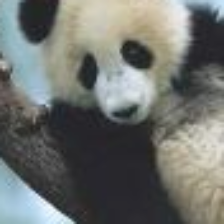
\includegraphics[width=.22\columnwidth]{adversarial-examples/panda_577.png} &%
			\centering\arraybackslash%
			$\centering +\ \epsilon \cdot$ &%
			
\includegraphics[width=.22\columnwidth]{adversarial-examples/nematode_082.png} &%
			$\centering =$ & %
			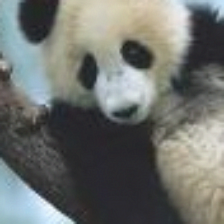
\includegraphics[width=.22\columnwidth]{adversarial-examples/gibbon_993.png} \\
			$\centering \vec x$     &%
			& $\sgn\del{\nabla_{\vec x} L(y,h(\vec x))}$ & & $\tilde{\vec x}$ \\
			\emph{panda} (0.577) & & & & \emph{gibbon} (0.993) 
		\end{tabular}
	}
	\caption{Generation of an adversarial example with FGSM, a single step attack. Italic words and numbers represent classes and confidences. The images are from \citet{Goodfellow:2014:EHAE}.}
	\label{fig:fgsm-adversarial-example}
\end{figure}

\paragraph{Transferability} An interesting property is that adversarial examples generated for one model are often misclassified by other models and models trained on different datasets, i.e. they generalize across models and datasets \citep{Szegedy:2013:IPNN}. This property of adversarial examples is called transferability. This suggests that most state-of-the art deep models are similarly biased. More analysis of transferebility can be found in \citet{Papernot:2016:TMLPBBAAS,Liu:2016:DTAEBBA,Tramer:2017:STAE}. 

\paragraph{Universal perturbations} \citet{Moosavi-Dezfooli:2016:UAP} have observed that there exist perturbations that can reliably produce adversarial examples when added to almost any input and hypothesize that they exploit geometric correlations between different parts of decision boundaries. 

\paragraph{Boundary tilting} \citet{Tanay:2016:ABTPPAE} hypothesize that adversarial examples exist when the decision boundary lies close to the submanifold of sampled data. They suggest that adversarial examples might be occurring along low-variance directions of the data where it is close to the manifold and that robustness could be improved with regularization. This is illustrated in figure \ref{fig:tanay-boundary-tilting}.

\begin{figure}[htbp!]
	\begin{center}
		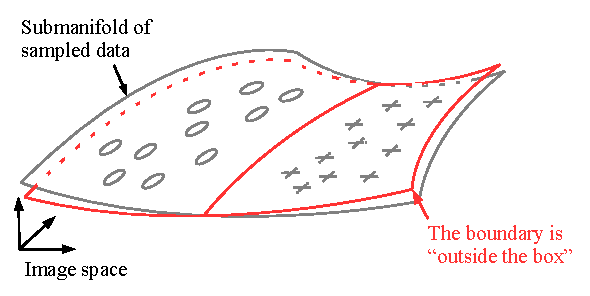
\includegraphics[width=\columnwidth]{figures/adversarial-examples/tanay-newPerspective.pdf}
	\end{center}
	\caption{An illustration of boundary tilting from \citet{Tanay:2016:ABTPPAE}.}
	\label{fig:tanay-boundary-tilting}
\end{figure}

\paragraph{High-dimensional space manifold geometry} \citet{Gilmer:2018:AS} hypothesize that the existence of adversarial examples could be a naturally occurring result of the geometry of high-dimensional data manifolds. For a simple dataset with two classes consisting of examples from a pair of high-dimensional concentric spheres, they have observed that most random points in the data distribution are both correctly classified and close to a misclassified point. The authors have also given negative evidence on the hypothesis that adversarial examples are off the data manifold by showing that \textit{on-manifold} adversarial examples can exist as well.

\paragraph{Adversarial examples of generative models} Adversarial examples are not just a phenomenon related to discriminative models. They have been found to exist for some generative models as well \citep{Goodfellow:2014:EHAE,Kos:2018:AEGM}. An example is shown in figure \ref{fig:vae-gan-targetad-face}.

\begin{figure}[htbp!]
	\begin{center}
		\raisebox{-0.5\height}{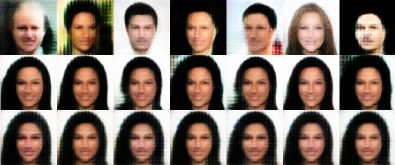
\includegraphics[scale=0.6]{figures/adversarial-examples/kos-exp11-faces-summary.png}}
		~
		\raisebox{-0.5\height}{
\includegraphics[scale=0.075]{figures/adversarial-examples/kos-exp11-faces-target-reconstruction.png}}
	\end{center}
	\caption{Reconstruction outputs for targeted attacks on a VAE-GAN model from \citet{Kos:2018:AEGM}. The rows represent of original image reconstructions (top), reconstructions of adversarial examples generated using an attack in latent space (middle) and a VAE-loss attack (bottom). The target reconstruction is on the right.}
	\label{fig:vae-gan-targetad-face}
\end{figure}

%\paragraph{Adversarial reprogramming.}

\paragraph{True ambiguity of adversarial examples of robust classifers}
Qualitative assesment of adversarial examples of robust classifiers suggest that they \textit{understand data} much better. Their adversarial examples really are ambigous, i.e. generated perturbations don't look like noise but are semantically meaningful to humans \citep{Tsipras:2018:RMBOA,Li:2019:AGCMRAA}.  This is illustrated in figures \ref{fig:tsipras-robust-adversarial-examples} and \ref{fig:li-gfz-adversarial-examples-mnist}. An interesting observation is that adversarially trained discriminative classifiers together with an iterative attack can interpolate between and generate quite realistic examples. \citet{Tsipras:2018:RMBOA} suggest a connection between the the saddle point problem of adversarial training and GAN training \citep{Goodfellow:2014:GAN}.

\begin{figure}[htbp!]
	\begin{center}
		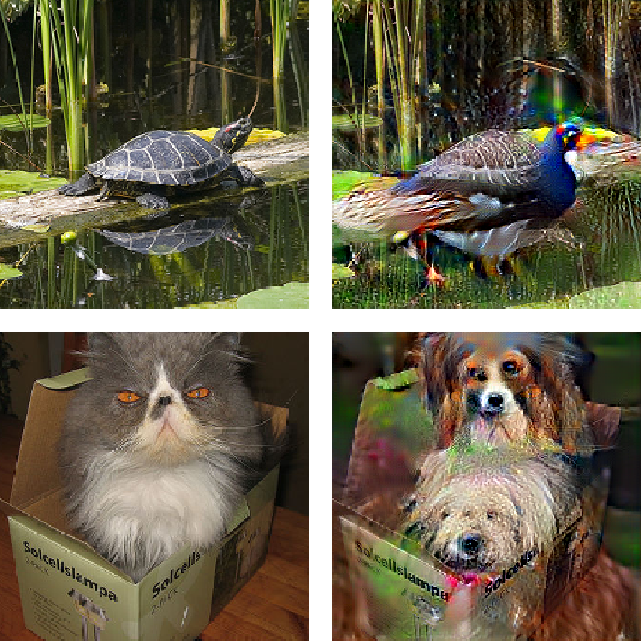
\includegraphics[width=0.85\columnwidth]{figures/adversarial-examples/tsipras-turtle-bird-cat-dogs}
	\end{center}
	\caption{Original images and adversarial examples generated with a large perturbation using an iterative non-targeted attack on an adversarially trained Restricted ImageNet \citep{Tsipras:2018:RMBOA} classifier from \citet{Tsipras:2018:RMBOA}.}
	\label{fig:tsipras-robust-adversarial-examples}
\end{figure}

\begin{figure}[htbp!]
	\begin{center}
		\raisebox{-0.5\height}{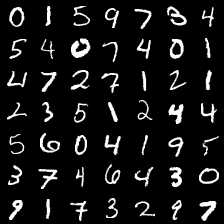
\includegraphics[scale=0.65]{figures/adversarial-examples/li-data_clean.png}}
		\
		\raisebox{-0.5\height}{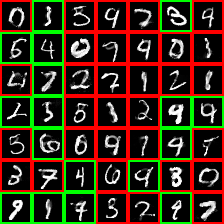
\includegraphics[scale=0.65]{figures/adversarial-examples/li-bayes_A_cw_adv.png}}
	\end{center}
	\caption{Clean images (left) and adversarial examples generated using an iterative non-targeted attack on a generative MNIST \citep{LeCun:2015:DL} classifier with the factorization $\p(\vec z)\p(\vec y\mid\vec z)\p(\vec x\mid\vec z,\vec y)$ (right) from \citet{Li:2019:AGCMRAA}. The adversarial examples marked in green are successful.}
	\label{fig:li-gfz-adversarial-examples-mnist}
\end{figure}

Further interesting phenomena and hypotheses related to the nature of adversarial examples, adversarial robustness and generalization will be discussed in section \ref{sec:robustness-generalization}.


\section{Finding adversarial examples} \label{sec:finding-adversarial-examples}

Let $\set X$ be the input space,
and $d\in(\set X\times\set X\to \R^+)$ a \textit{distance function} for definining similarity between inputs. 
For each example $\vec x$, 
we can also define its \textit{neighbourhood} as $B_{\epsilon}(\vec x) = \cbr{\vec x'\colon d(\vec x', \vec x) \leq \epsilon}$,
where $\epsilon$ is the maximum distance from the example.

Ideally, the neighbourhood of an example $\vec x$ should be the set of \textit{perceptually similar} examples that all belong to the same class as $\vec x$ (their true class may be at most ambiguous), but it is hard to define such a neighbourhood (as it requires knowing the true model). A practical and common way of defining the neighbourhood function for images is to have $d$ be a $L^p$ distance where $p$ is usually $\infty$ or $2$. Note that, if an example is very near the true class boundary, such a neighbourhood may contain examples belonging to another class. 

\subsection{Attack objectives}

Finding an adversarial example can be defined as a constrained optimization problem of maximizing some loss with respect to the input with the constraint that the input is in the neighbourhood $B_\epsilon(\vec x)$:
\begin{align}
\tilde{\vec x} = \argmax_{\vec x'\in B_\epsilon(\vec x)} L(y, h(\vec x')) \text{,} \label{eq:non-targeted-loss-attack}
\end{align}
where $y$ is the true label. Let $\hat{h}(\vec x) \coloneqq \argmax_{y} h(\vec x)_\ind{y}$ denote the function that assigns the label with the highest probability to an input.
An objective can also be to find the $\tilde{\vec x}$ closest to $\vec x$ such that the classifier misclassifies it \citep{Moosavi-Dezfooli:2016:DFSAMFDNN}:
\begin{align}
\tilde{\vec x} = \argmin_{\vec x'\colon \vec x'\in B_\epsilon(\vec x) \land \hat{h}(\vec x') \neq y} d(\vec x', \vec x) \text{.} \label{eq:non-targeted-closest-attack}
\end{align}

The described objectives, where it only matters that the adversarial example is misclassified, are objectives for \textit{non-targeted adversarial attacks}. There are also \textit{targeted adversarial attacks}, where the objective is to create an adversarial example such that the model classifies it as some desired target. Targeted attack objectives corresponding to equations \eqref{eq:non-targeted-loss-attack} and \eqref{eq:non-targeted-closest-attack} are:
\begin{align}
\tilde{\vec x} &= \argmin_{\vec x'\in B_\epsilon(\vec x)} L(y_\text{a}, h(\vec x')) \text{,} \label{eq:targeted-loss-attack} \\
\tilde{\vec x} &= \argmin_{\vec x'\colon \vec x'\in B_\epsilon(\vec x) \land \hat{h}(\vec x') = y_\text{a}} d(\vec x', \vec x) \text{,} \label{eq:targeted-closest-attack}
\end{align}
where $y_\text{a}$ denotes the adversarial target label. The difference in equation \eqref{eq:targeted-loss-attack} is loss minimization and the adversarial target label instead of the true label. The difference in equation \eqref{eq:targeted-closest-attack} is the condition that the predicted labels equals the adversarial target instead of differing from the true label.

non-targeted adversarial examples can also be generated without knowledge of the true label. Instead of the true label $y$, the predicted label $\hat{h}(\vec x)$ can be used in equations \eqref{eq:non-targeted-loss-attack} and \eqref{eq:non-targeted-closest-attack}. Such adversarial examples are called \textit{virtual adversarial examples}.
\citet{Miyato:2017:VATRMSSSL} propose the following attack objective for use in semi-supervised learning:
\begin{align}
\tilde{\vec x} = \argmin_{\vec x'\in B_\epsilon(\vec x)} D((\rvar y\mid \vec x, \vec\theta), (\rvar y\mid \rvec x = \vec x', \vec\theta)) \text{,}
\end{align}
where $D$ is some non-negative function that represents distance between distributions.

For adversarial training, non-targeted attacks should be preferred due to the \textit{label-leaking} phenomenon \citep{Kurakin:2016:AMLS} where the learned classifier can overfit to adversarial examples and perform better on them than on natural examples, especially with attacks with a small number of iterations. For robustness evaluation with datasets that have many similar classes, non-targeted attacks can too easily fool the classifier and targeted attacks give more meaningful evaluation results \citep{Athalye:2018:OGGFSS}.

\subsection{Common attacks}

Being that finding adversarial examples is a constrained optimization problem, general gradient-based and black-box optimization algorithms can be used for attacks. Additionally, sometimes techniques specific to some potential defense and machine learning algorithm have to be used.

Some commonly known gradient-based attacks for finding adversarial examples are the following (using the notation from section \ref{sec:finding-adversarial-examples}):
\begin{itemize}
	\item Box-constrained L-BFGS -- \citet{Szegedy:2013:IPNN} propose to minimize $c\enVert{\vec x -\tilde{\vec x}}_2^2+L(y,h(\tilde{\vec x}))$ with the constraint $\tilde{\vec x}\in\intcc{0,1}$ with L-BFGS, a quasi-Newton optimization method. $c$ is a number obtained via line-search that yields adversarial examples of minimum distance.
	\item Fast gradient sign method (FGSM) -- an attack proposed by \citet{Goodfellow:2014:EHAE} that requires a single gradient computation:
	\begin{align}
	\tilde{\vec x} = \vec x + \epsilon\nabla_{\vec x} L(y,h(\vec x)) \text{,}
	\end{align} 
	where $\epsilon$ is the $L^\infty$-norm of the perturbation. For $L^2$-constrined perturbations, \citet{Miyato:2017:VATRMSSSL} propose $L^2$ normalization instead of the sign function.
	\item DeepFool -- an iterative non-targeted attack proposed by \citet{Moosavi-Dezfooli:2016:DFSAMFDNN} that in each step finds the optimal solution to a linear approximation of a loss in the $L^2$ ball $B_\epsilon(\vec x)$ using the gradient in the current adversarial input. It is faster and finds smaller perturbations than L-BFGS and stronger than FGSM.
	\item Projected gradient descent (PGD) \citep{Madry:2017:TDLMRAA} basic iterative method (BIM) \citep{Kurakin:2016:AEPW} -- an iterative gradient-based algorithm with random initialization \citep{Madry:2017:TDLMRAA} of the perturbation from within the $B_\epsilon(\vec x)$ at the start and steps in the direction of the gradient sign:
	\begin{equation} \label{eq:pgd}
	\tilde{\vec x}_i = \Pi_{B_\epsilon(\vec x)} \del{\tilde{\vec x}_{i-1} + \alpha\sgn\del{\nabla_{\tilde{\vec x}_{i-1}} L(y,h(\tilde{\vec x}_{i-1}))}} \text{.}
	\end{equation}
	$\alpha$ is the step size, and $\Pi_{B_\epsilon(\vec x)}$ is the projection into the $L^p$ $\epsilon$-ball around $\vec x$.
	\item Carlini-Wagner (CW) attacks -- \citet{Carlini:2017:TERNN} propose attacks with similar minimal perturbation objectives as \citet{Szegedy:2013:IPNN} and \citet{Moosavi-Dezfooli:2016:DFSAMFDNN}. They modify the loss function and, to enable unconstrained optimization, they introduce change of variables $\vec\delta=\frac{1}{2}\del{\tanh\del{\vec w} + \cvec 1} - \vec x$, which limits the perturbation $\vec\delta$ to the interval $\intcc{0,1}$. With the PGD (BIM) attack, it is currently probably one of the 2 strongest attacks.
\end{soliditemize}


\section{Improving adversarial robustness}

There are different approaches (\textit{defenses}) trying to improve adversarial robustness, most of which have been shown to actually be non-robust, but had appeared robust because they intentionally or unintentionally caused attacks that they were evaluated on not to be able to find adversarial examples \citep{Carlini:2017:AEANEDBTM,Athalye:2018:OGGFSS,Uesato:2018:ARDEAWA,Carlini:2017:TERNN}.  Thus, it is important to put as much effort as needed to correctly evaluate robustness, i.e. get an as low as possible upper bound on robustness. \citep{Carlini:2019:OEAR} is a recent helpful overview on evaluation of robustness. 

A broad overview of many defenses can be found in \citet{Serban:2018:AECCP}. To give a few examples, some approaches use generative models to approximately project inputs to a learned data manifold (e.g. \citet{Samangouei:2018:DGPCAAAUGM}), some approaches are based on limiting the Lipschitz constant of the model to limit sensitivity to small input perturbations by regularization and model modification (e.g. \citet{Qian:2018:L2NNN}), some research is looking into ways of guaranteeing robustness (e.g. \citet{Cohen:2019:CARRS}).

\subsection{Adversarial training and empirical adversarial risk}

The only defense currently believed to be effective according to \citet{Athalye:2018:OGGFSS} is adversarial training \citep{Goodfellow:2014:EHAE} with a strong attack \citep{Madry:2017:TDLMRAA}, where the model is trained on adversarial examples as well as natural examples.

\citet{Madry:2017:TDLMRAA} define what can be called \textit{empirical adversarial risk} by allowing the worst-case attack to modify each the input in the empirical risk expression:
\begin{align}
R_\text{EA}(h,\set D) \coloneqq \E_{(\vec x, y)\sim p_{\set D}} \del{\max_{\tilde{\vec x}\in B_\epsilon(\vec x)} L(y,h(\tilde{\vec x}))} \text{.}
\end{align}
They propose PGD for the attack during training and PGD with as large a number of iterations as necessary to approximate the worst-case adversary, i.e. get a better upper bound on robustness.

Still, adversarially trained models are not robust to attacks with weaker constraints than those used for training \citep{Schott:2018:TDFARNNMM}. Furthermore, because adversarial examples are generated and robustness is evaluated according to the practical definition of an adversarial example and using $L^p$ distance as a non-ideal approximation of perceptual similarity, performance is affected \citep{Madry:2017:TDLMRAA,Tsipras:2018:RMBOA} and there can exist misclassified examples among which are \textit{invariance-based} adversarial examples \citep{Jacobsen:2019:EEICNBAR}.

%Empirical and theoretical results show that improving robustness seems to be a problem that requires more model capacity and causes a reduction of performance on natural data \citep{Madry:2017:TDLMRAA,Tsipras:2018:RMBOA}.


\section{Adversarial robustness and generalization} \label{sec:robustness-generalization}

Based on the practical definition of an adversarial example or similar definitions, experimental \citep{Madry:2017:TDLMRAA,Su:2018:IRTCOACSRDICM} and theoretical evidence \citep{Tsipras:2018:RMBOA} suggests that there is a trade-off between robustness and standard generalization for current models.

Here are some recent discoveries related to adversarial robustness and generalization presented. Robustness to distributional shift and corruptions also seems to be quite relevant \citep{Gilmer:2019:AENCTEN,Hendrycks:2019:BNNRCCP}, but it will not be discussed here.

\subsection{A trade-off between robustness and generalization}

\citet{Madry:2017:TDLMRAA,Su:2017:OPAFDNN,Tsipras:2018:RMBOA} and others have empirically observed that adversarial robustness with current algorithms requires more capacity and negatively affects generalization. \citet{Su:2017:OPAFDNN} have observed that older convolutional architectures with no shortcut connections, like AlexNet \citep{Krizhevsky:2012:ICDCNN} and VGG \citep{Simonyan:2014:VDCNLSIR} seem to be inherently more robust than architectures like ResNet \citep{He:2015:DRLIR}, DenseNet \citep{Huang:2016:DCCN} and MobileNet \citep{Howard:2017:MECNNMVA} and NASNets \citep{Zoph:2018:LTASIR} with standard training. \citet{Madry:2017:TDLMRAA} has observed that with adversarial training, more model capacity is required and natural test set performance is reduced. Furthermore, \citet{Tsipras:2018:RMBOA} have, based on the practical definition of an adversarial example, theoretically demonstrated an aspect of the trade-off. Another reason that affects performance suggested by them is that salient features might be harder to learn and that algorithms rely on highly predictive but \textit{non-robust} features.

\subsection{Non-robust features}

Based on some ideas from \citet{Tsipras:2018:RMBOA},  \citet{Ilyas:2019:AENBTF} propose an interesting and experimentally well supported hypothesis on the nature of features that well-generalizing non-robust classifiers learn. They show that existence of adversarial examples can be directly attributed to existence of  non-robust features, "features derived from patterns in the data that are highly predictive but brittle and incomprehensible to humans". 

They demonstrate the predictiveness of non-robust features by: 
\begin{solidenumerate}
	\item constructing a dataset $\set D_\text{NR}$ where approximately the only useful features are non-robust features by turning inputs of the original dataset $\set D$ into adversarial examples for a classifier that was trained standardly and relabeling them with the adversarial label,
	\item training a new classifier on the non-robust dataset $\set D_\text{NR}$,
	\item testing the new classifier on the original test set where it achieves performance close to the original classifier and lower robustness.
\end{enumerate}

In another experiment, they try to remove non-robust-features from inputs with the help of an adversarially trained classifier. A new classifier trained on the dataset with removed non-robust features achieves a bit lower performance and robustness not as high as the adversarially trained classifier but quite significant compared to the standardly trained classifier. Results of these experiments with the CIFAR-10 dataset \citep{Krizhevsky:2009:LMLFTI} are shown in figure \ref{fig:iliyas-experiment-results}.

\begin{figure*}[htbp!]
	\centering
	\begin{subfigure}[b]{0.45\textwidth}
		\centering
		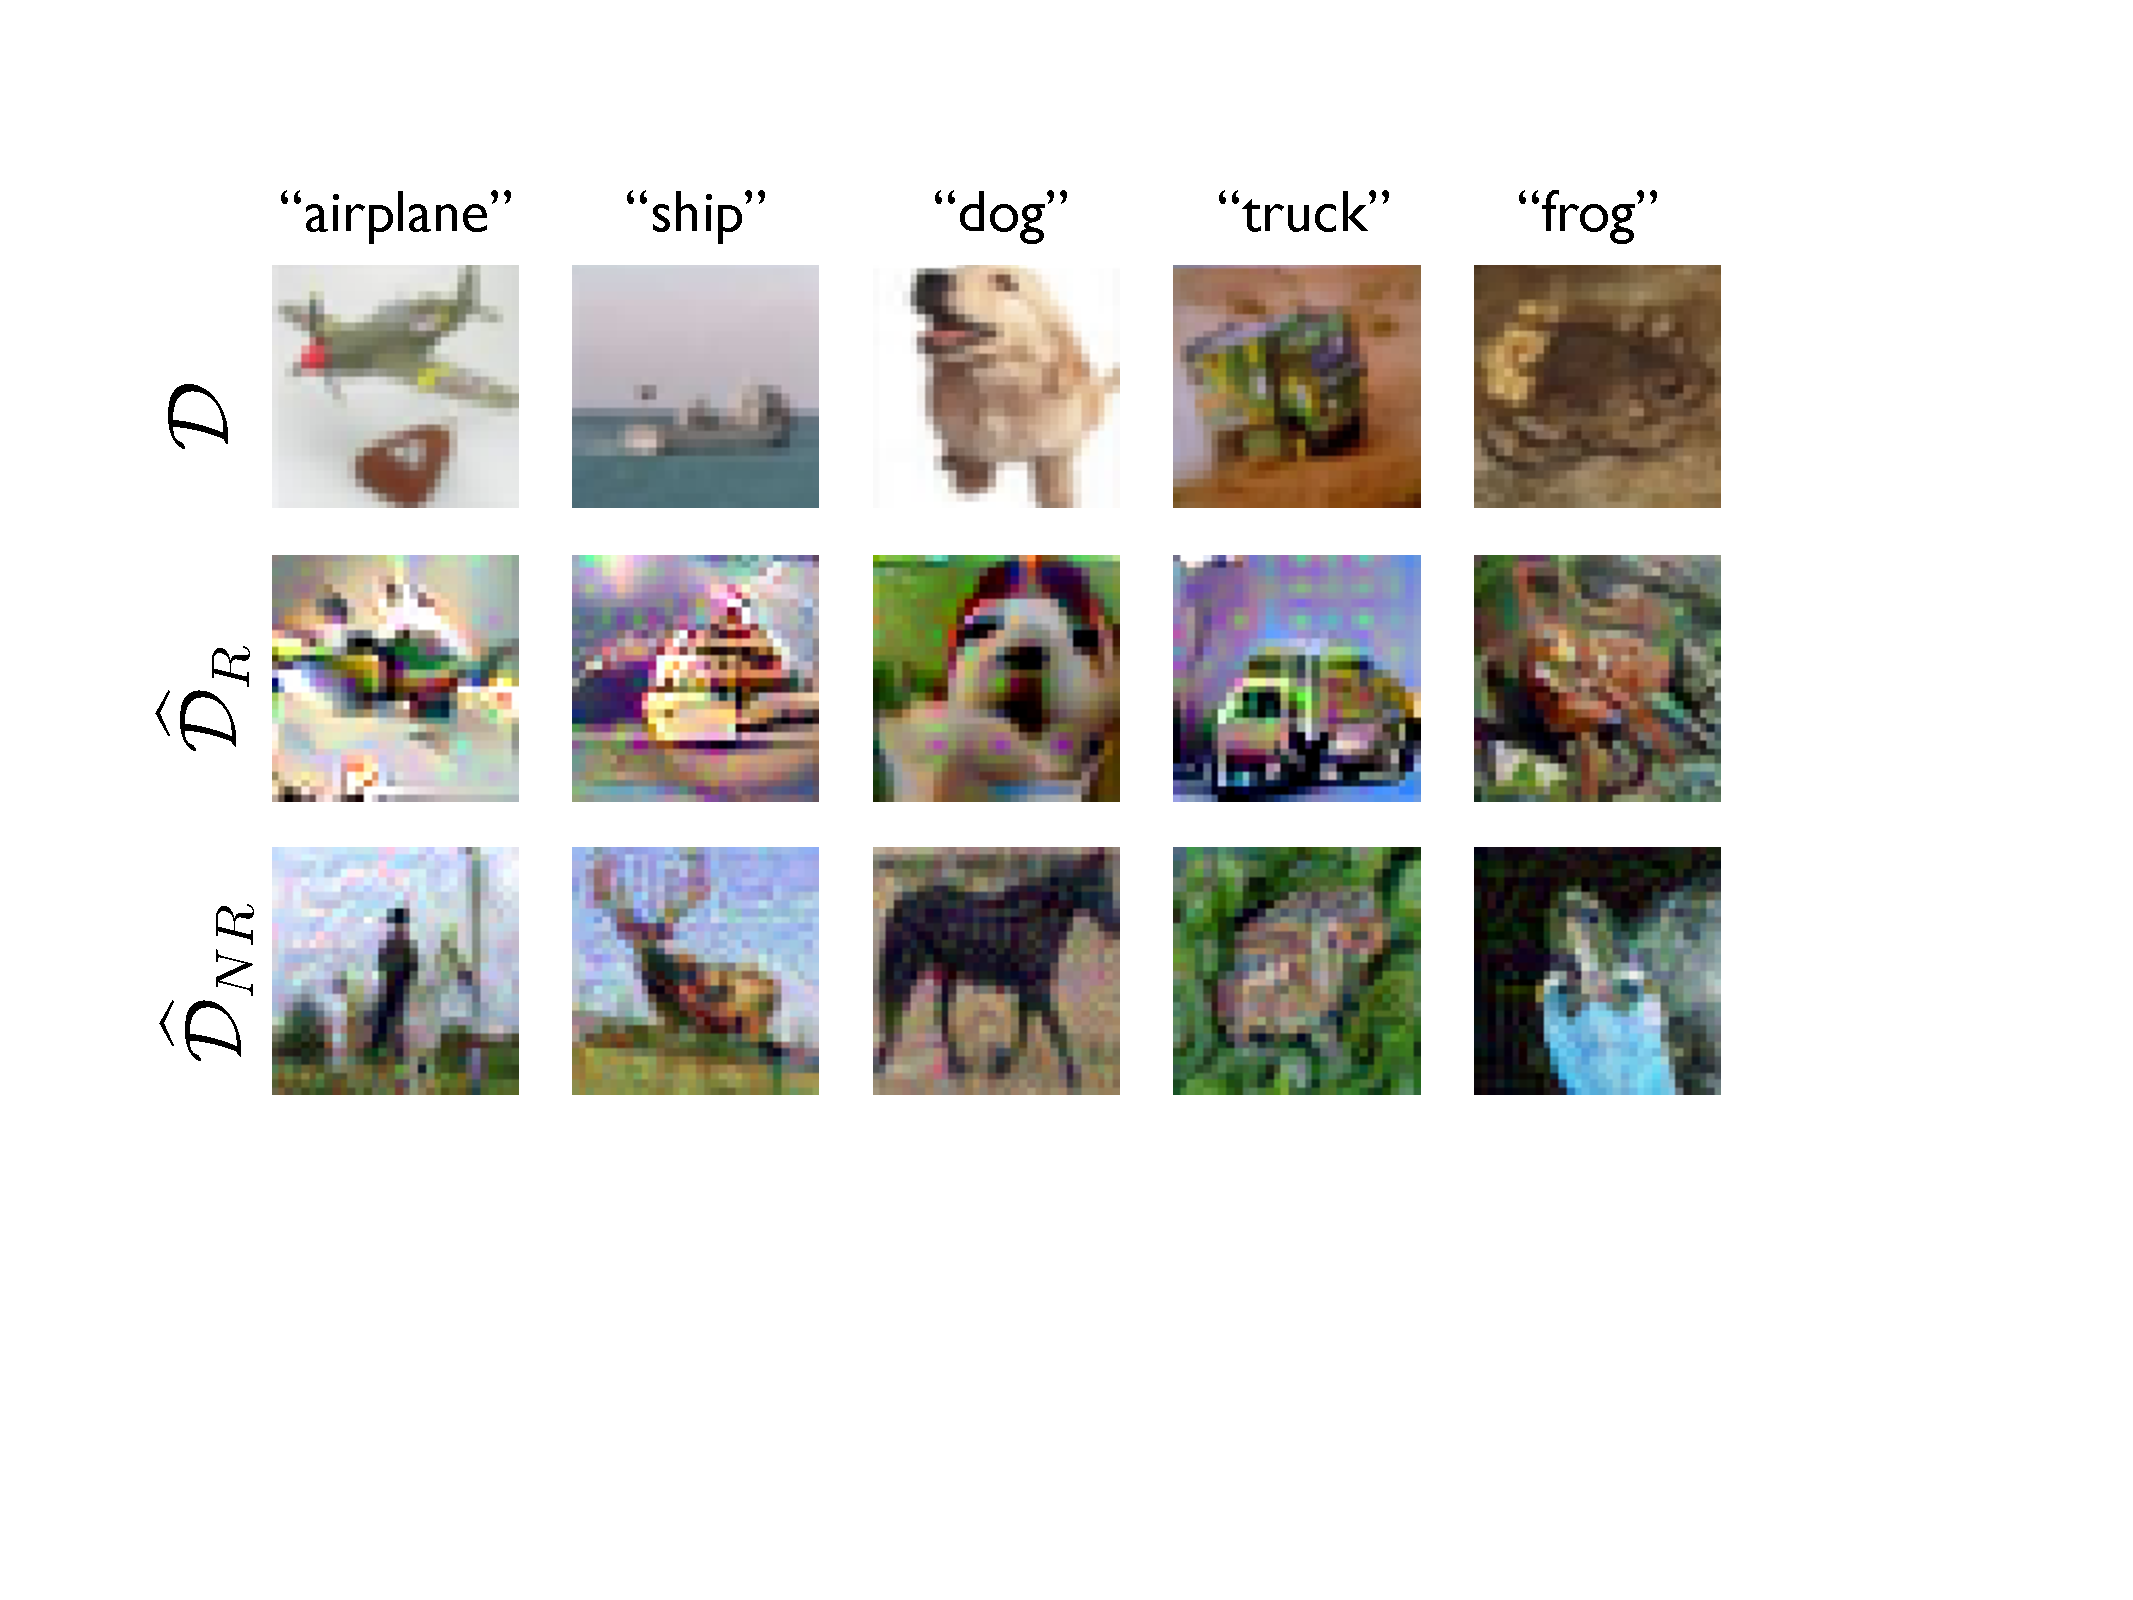
\includegraphics[width=1.0\textwidth]{figures/adversarial-examples/ilyas/cifar_datasets.pdf}
		\vfill\null
		\caption{}
		\label{fig:robust_inputs}
	\end{subfigure}
	\hfill
	\begin{subfigure}[b]{0.5\textwidth}
		\centering
		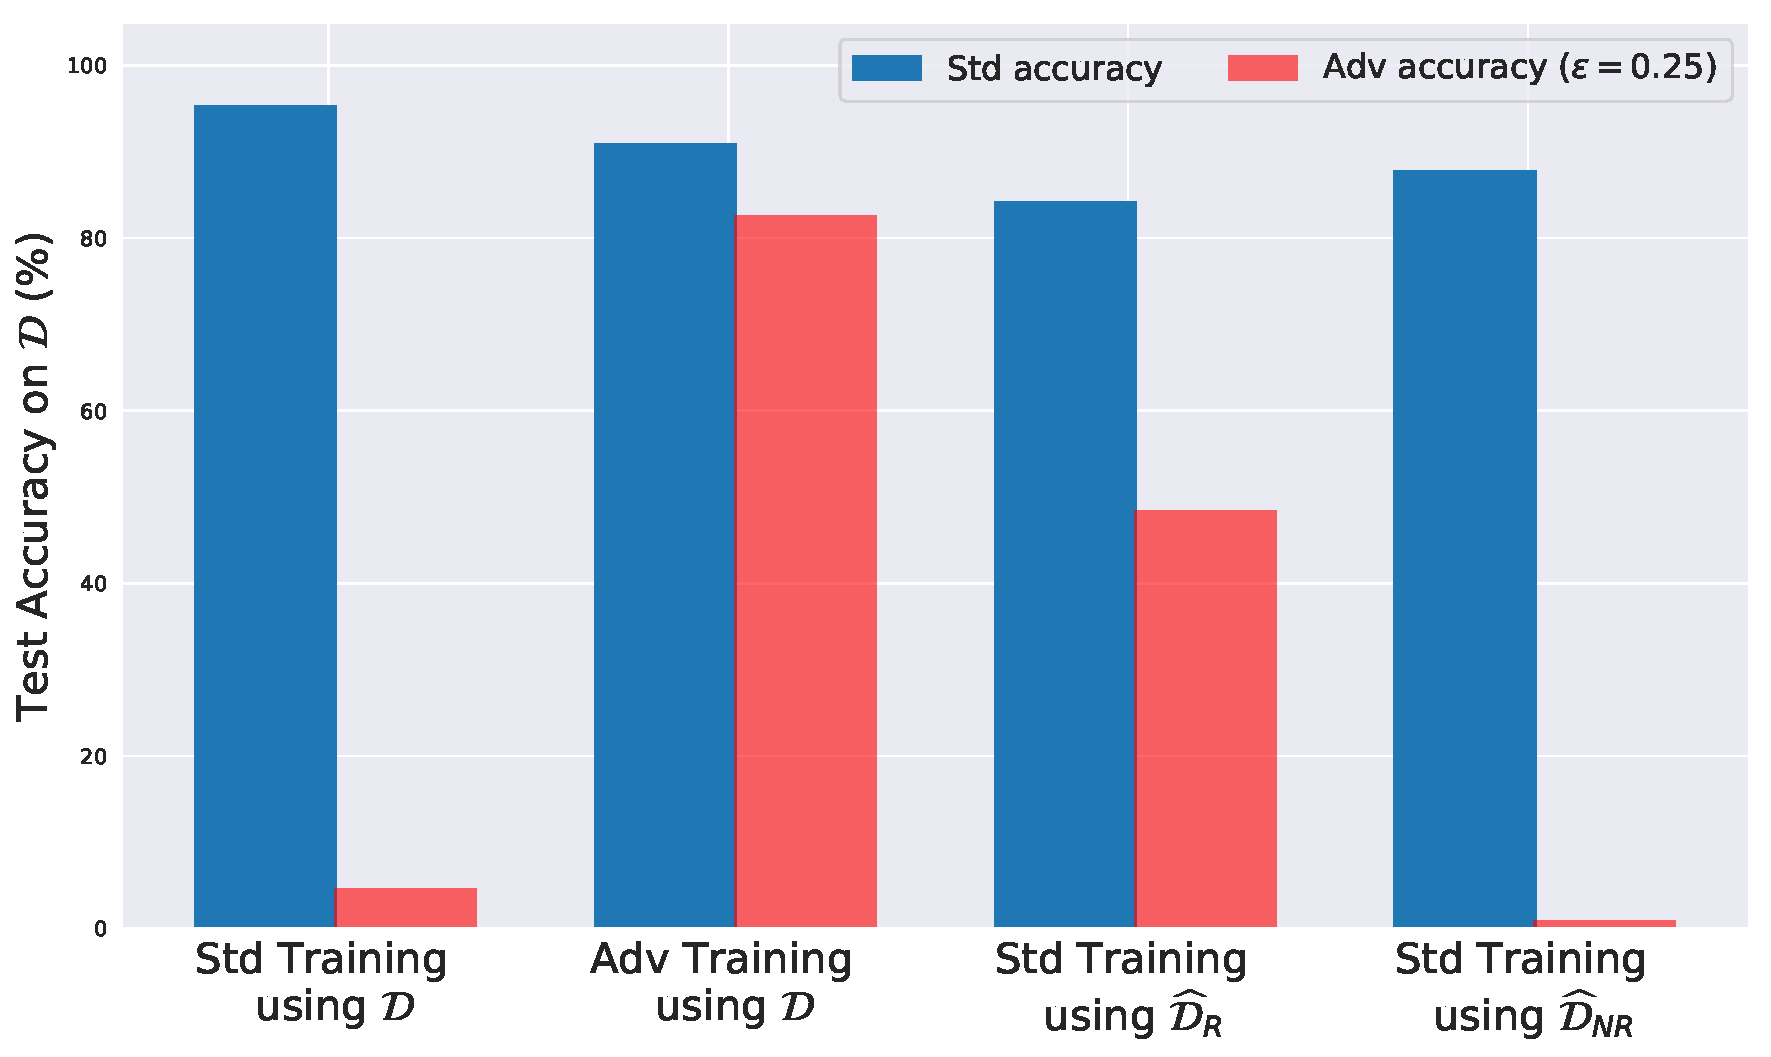
\includegraphics[width=\textwidth]{figures/adversarial-examples/ilyas/CIFAR_res.pdf}
		\caption{}
		\label{fig:robustify_cifar}
	\end{subfigure}
	\caption{
		(a) Random samples from variants of the
		CIFAR-10 training set:
		the original training set; 
		the \textit{robust training set} $\set D_\text{R}$, restricted to features used by a
		robust model; and
		the \textit{non-robust training set} $\set D_\text{NR}$, restricted to
		features relevant to a standard model (labels appear incorrect to humans).
		(b) Standard and robust accuracy on the CIFAR-10
		test set ($\set D$) for models trained with standard training, adversarial training, and standard training on datasets $\set D_\text{R}$ (robust) and $\set D_\text{NR}$ (non-robust). Adapted from \citet{Ilyas:2019:AENBTF}.}
	\label{fig:iliyas-experiment-results}
\end{figure*}

\subsection{Training with on-manifold adversarial examples}

\citet{Stutz:2018:DARG} challenge the hypothesis that there is a trade-off between robustness and generalization. They hypothesize that most adversarial examples come from directions orthogonal to the learned class manifolds and that training adversarial examples (as per a definition similar to definition \ref{def:ae-consistent}) limited to the known or learned class manifolds (on-manifold adversarial examples) can improve generalization. They conduct experiments with a synthetic dataset with known class-invariant transformations and datasets with small images that support the hypothesis that generalization can be improved with adversarial training with on-manifold adversarial examples.

Class manifolds to which adversarial examples are restrited and on-manifold and off-manifold adversarial examples are illustrated in figure \ref{fig:stutz-illustration}.

\begin{figure}[htbp!]
	\begin{center}
		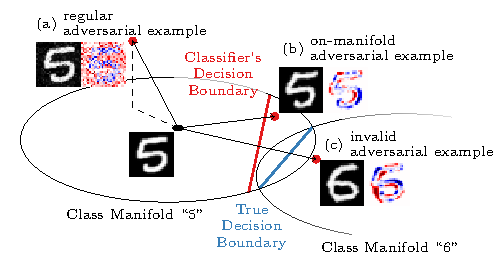
\includegraphics[width=\columnwidth]{figures/adversarial-examples/stutz-introduction_b.pdf}
	\end{center}
	\caption{An illustration by \citet{Stutz:2018:DARG} of class manifolds (classes "5" and "6") with a regular (off-manifold) adversarial example and an on-manifold adversarial example.}
	\label{fig:stutz-illustration}
\end{figure}

In one of the experiments \citet{Stutz:2018:DARG} construct a synthetic dataset with a known manifold (geometric transformations of letters) in order to be able to generate exactly on-manifold adversarial examples by modifying parameters of the geometric transformations. With this dataset, they succeed in improving generalization and on-manifold robustness\footnote{By the authors' definition of an adversarial example, which is similar to the consistent definition (definition \ref{def:ae-consistent}), except for that there is no closeness constraint, making it equivalent to the definition of a misclassified example, on-manifold robustness essentially boils down to generalization.} with adversarial training.

In other experiments they use EMNIST \citep{Cohen:2017:EMNIST}, FashionMNIST \citep{Xiao:2017:FMNIDBMLA} and CelebA \citep{Liu:2015:DLFAW}. In order to better approximate class manifolds and disable leaving the manifold of a class when an adversarial example is generated for adversarial training, they first train one variational autoencoder (VAE-GAN) per class. They perform training and evaluation analogously to the experiment with synthetic data by allowing the attack to perturb the latent representation of the autoencoder corresponding to the correct class. They measure positive correlation between robustness to on-manifold adversarial examples and generalization. They observe worse quality of on-manifold adversarial examples for the more complex dataset CelebA due to worse approximation quality of their VAE-GAN-s.


\section{Conclusion}

This paper presents an overview of ideas related to the existence adversarial examples, hypotheses on their existence and some of their properties. It describes general principles regarding adversarial attacks, defenses and robustness evaluation and presents examples of such algorithms. Finally, some recent discoveries and hypotheses regarding the relation between robustness and generalization are explored. Some recent results \citep{Stutz:2018:DARG} suggest that finding ways of improving both robustness generalization might be an interesting research direction to explore.


\newpage.
\newpage

 Adversarially robust generalization requires
more data show 

distilling knowledge into a small dataset

With some reasonable assumptions about the model, as the model approaches the true model (in robustness/), its (/on-manifold) adversarial examples would be becoming more close to the true decision boundary, i.e. truly more ambigous (/more often actually changing the class). The true model has no on-manifold adversarial examples, but it might not be defined for off-manifold examples, e.g. if it is a discriminative model.



\newpage

\subsection{Robustness evaluation}

\citet{Athalye:2018:OGGFSS} state that, if there are classes that are very similar, using targeted attacks for robustness evaluation can give more meaningful results. 

stronger attack targeted, stronger evaluation untargeted

\subsubsection{Adversarial training}

\citet{Kurakin:2016:AMLS} note that by using the true label in the loss in untargeted attacks ($y$ in equation \eqref{eq:untargeted-loss-attack}) can cause


\newpage
.
\newpage
\subsubsection{Distance metrics for images}

Usually, an $L^p$ distance ($d(\vec x', \vec x)=\lVert\tilde{\vec x}-\vec x\rVert_p$) is used as a distance metric for adversarial examples.

\paragraph{Scale-invariant norms.}
Let $\vec x$ denote some image (or perturbation) and $\vec x_\lambda$ the same image with dimensions scaled by $\lambda$. $\vec x_\lambda$ has a greater norm because it contains $\lambda^2$ the number of pixels of the original image and every pixel is approximately effectively repeated $\lambda^2$ times. In terms of $\enVert{\vec x}_p$, its norm can be approximated like this:
\begin{align*}
    \enVert{\vec x_\lambda}_p 
    &= \del{\sum_{u\in\cbr{0\bidot\lambda H}}\sum_{v\in\cbr{0\bidot\lambda W}} \envert{{\vec x_\lambda}_\ind{u, v}}^p}^{\frac{1}{p}} && \text{(norm definition)} \\
    &\approx \del{\sum_{u\in\cbr{0\bidot H}}\sum_{v\in\cbr{0\bidot W}} \lambda^2 \envert{{\vec x}_\ind{u, v}}^p}^{\frac{1}{p}} && \text{($\lambda^2$ element copies)} \\
    &= \lambda^\frac{2}{p} \del{\sum_{u\in\cbr{0\bidot H}}\sum_{v\in\cbr{0\bidot W}} \envert{{\vec x}_\ind{u, v}}^p}^{\frac{1}{p}} \\
    &= \lambda^\frac{2}{p} \enVert{\vec x}_p \text{.} && \text{(norm definition)}
\end{align*}

If there is a perturbation in $2$ different resolutions, the higher-resolution one will have a greater norm by approximately a factor of $(\lambda^2)^\frac{1}{p}$, especially if the perturbations don't have too high spatial frequencies. Hence, scale invariant equivalents of $L^p$ norms can be defined by dividing the norm by the scale factor. If we choose the scale factor to be relative to the scale of an image with area $1$, $\lambda^2$ is $n$, the total number of pixels. 

We can define \textbf{scale-invariant norms} like this:
\begin{align}
    \mathrm{m}_p(\vec x) \coloneqq n^{-\frac{1}{p}}\enVert{\vec x}_p, \label{eq:scale-invariant-norm}
\end{align}
This can also be expressed as the \textbf{generalized mean} $\mathrm{M}_p$ (also known as \textbf{power mean}) of the elementwise absolute value:
\begin{align}
    \mathrm{m}_p(\vec x) = \mathrm{M}_p(\envert{\vec x}) \coloneqq \del{\frac{1}{n}\sum_i  \envert{\vec x_\ind{i}}^p}^{\frac{1}{p}}. \label{eq:generalized-mean}
\end{align}
Such norms could probably be useful for comparison of norms between different-resolution images and different datasets, and hyperparameter choice for adversarial attacks.

Maybe something similar could be done about objects of different scale?

...

\paragraph{Expectation of scale-invariant norms uniformly distributed random vectors.}
Let $\rvec x_n$ be a random vector with $n$ independent elements ${\rvec x_n}_\ind{i}\sim\mathcal{U}\del{\intcc{-\epsilon,\epsilon}}$.

An easy special case is when $p=1$:
\begin{align*}
    \E\sbr{\mathrm{m}_1(\rvec x_n)}
	= \E\sbr{\frac{1}{n}\sum_i \envert{{\rvec x_n}_\ind{i}}}
	= \E\sbr{\envert{{\rvec x_n}_\ind{i}}}  
	= \frac{\epsilon}{2} \text{.}
\end{align*}

For very large $n$, we can approximate it like this:
\begin{align*}
	\lim_{n\to\infty} \E \sbr{\mathrm{m}_p(\rvec x_n)}
	&= \E\sbr{\lim_{n\to\infty}\del{\frac{1}{n}\sum_i \envert{{\rvec x_n}_\ind{i}}^p}^\frac{1}{p}} &&\text{(dominated convergence)} \\
	&= \E\sbr{\E\sbr{\envert{{\rvec x_n}_\ind{0}}^p}^\frac{1}{p}} &&\text{(IID elements)}  \\
	&= \E\sbr{\envert{{\rvec x_n}_\ind{0}}^p}^\frac{1}{p} &&\text{(redundant expectation)}  \\
	&= \frac{1}{2\epsilon} \del{\int_{-\epsilon}^{\epsilon}\envert{x}^p\dif x}^\frac{1}{p} &&\text{(definition of expectation)}  \\	
	&= \frac{1}{\epsilon}\del{\int_{0}^{\epsilon}x^p\dif x}^\frac{1}{p} &&\text{(absolute value symmetry)}  \\	
	&= \frac{1}{\epsilon}\del{\frac{\epsilon^{p+1}}{p+1}}^\frac{1}{p} \text{.} \numberthis\label{eq:power-norm-n-infinity}
\end{align*}
Specially, for $\epsilon=1$, it evaluates to 
\begin{align}
	 \lim_{n\to\infty} \E \sbr{\mathrm{m}_p(\rvec x_n)} = (p+1)^{-\frac{1}{p}} \text{.}
\end{align}

TODO: Show that \eqref{eq:power-norm-n-infinity} is the upper bound if $p>1$ and the lower bound if $p<1$.

By the power mean inequality, which can be proved by applying the Jensen inequality, $\mathrm{m}_p(\rvec x)$ is monotonically increasing in $p$ (for $p>0$).


For easier analysis, let's first consider a special case: ${\rvec x_n}_\ind{i}\sim\mathcal{U}\del{\intcc{0,1}}$.
\begin{align*}
	\E \sbr{\mathrm{m}_p(\rvec x_n)}
	&= \E\sbr{\del{\frac{1}{n}\sum_i \envert{{\rvec x_n}_\ind{i}}^p}^\frac{1}{p}}  \\
	% not good (no dependence on n): &\approx \E\sbr{\del{\frac{1}{2p}}^\frac{1}{p}}  \\
	&= \idotsint_{\intcc{0,1}^n} \del{\frac{1}{n}\sum_i \envert{\vec x_\ind{i}}^p}^\frac{1}{p} \dif\vec x  \\
	&= n^{-\frac{1}{p}}\idotsint_{\intcc{0,1}^n} \del{\sum_i \envert{\vec x_\ind{i}}^p}^\frac{1}{p} \dif\vec x  
\end{align*}


\paragraph{Local $p$-norm and hiererchical norm.}
Let $\vec k$ denote a non-negative $2$-D kernel with $\enVert{\vec k}_1=1$, e.g. Gaussian cenetered at $(0,0)$. Let $\vec x$ denote an image perturbation and assume that it has a single channel for simplicity.
We can define the local $p$-norm around a pixel $(i, j)$ as
\begin{align}
    \mathrm{LocalNorm}_{p,\vec k}(\vec x)_\ind{i,j} = \del{\envert{\vec x}^p * \vec k}_\ind{i,j}^\frac{1}{p},
\end{align}
where the absolute value and powering operatons are elementwise.

We can then define a bi-level hierarchical $(p_1,p_2)$-norm as $\enVert{\mathrm{LocalNorm}_{p_1,\vec k}(\vec x)}_{p_2}$. This can be generalizad to a multi-level norm $(p_1,..,p_n)$-norm by chaining multiple local norms with potentially different kernels until the last, global, $p_n$-norm.

Why?

%Using e.g a $(1,\infty)$-norm for contraining adversarial perturbations could allow for more flexible perturbations locally, but having local changes not add up to the global norm.

%To make the analysis easier, we can consider $\vec x$ and $\vec x_\lambda$ to be continous functions with delta-peaks at the coordinates of pixels. 

%\begin{align}
%    \enVert{\vec x_\lambda}_p = \del{ \int_{u\in\intcc{0,\lambda h}\cap\N}\int_{v\in\intcc{0,\lambda w}\cap\N} {\vec x_\lambda}\del{u, v}}^{\frac{1}{p}}
%\end{align}


\chapter{Other}


\part{Generative models}



\section{Generative adversarial networks}

\subsection{Getting the probability of the example from the generator}

first paragraph

case 1) normal generator

case 2) invertible generator




\part{Ideas from papers and paper summaries}



\section{Ideas from papers}

\subsection{Excessive Invariance Causes Adversarial Vulnerability}

\citet{Jacobsen:2019:EEICNBAR}:
\begin{itemize}
    \item \say{We hypothesize that a major reason for this excessive invariance can be understood from an information-theoretic viewpoint of cross entropy, which maximizes a bound on the mutual information between labels and representation, giving no incentive to explain all class-dependent aspects of the input. This may be desirable in some cases, but to achieve truly general understanding of a scene or an object, machine learning models have to learn to successfully separate essence from nuisance and subsequently generalize even under shifted input distributions.}
    \item \say{All adversarial examples can be reached either by crossing the decision-boundary of the classifier via perturbations, or by moving within the pre-image of the classifier to mis-classified regions. The two viewpoints are complementary to one another and highlight that adversarial vulnerability is not only caused by excessive sensitivity to semantically meaningless perturbations, but also by excessive insensitivity to semantically meaningful transformations.}
\end{itemize}

\subsection{You Only Propagate Once: Accelerating Adversarial
Training via Maximal Principle}




\section{Paper summaries}

\subsection{The Conditional Entropy Bottleneck (Anonymous, 2018)}

URL: \url{https://openreview.net/forum?id=rkVOXhAqY7}.


\section{p}

Neka je odnos između slučajnih varijabli $\rvar x$ i $\rvar y$ definiran funkcijom $f$ koja ishode jedne slučajne varijable deterministički preslikava u ishode druge, što označavamo ovako: $\rvar y = f(\rvar x)$.  Ako su $\rvar x$ i $\rvar y$ diskretne slučajne varijable, onda je razdioba slučajne varijable $\rvar y$ definirana ovako:
\begin{align}
	P_{\rvar y}(y) = \sum_{x\colon f(x)=y} P_\rvar{x}(x) \text{.}
\end{align} 
Ako su $\rvar x$ i $\rvar y$ kontinuirane slučajne varijable s vrijednostima iz $\R$ i $f$ je injektivna, može se pokazati \citep{Elezovic:2007:VSSV} da vrijedi
\begin{align} \label{eq:gustoca-funkcije-sv}
p_{\rvar y}(y) = p_\rvar{x}(x) \envert{\od{x}{y}} \text{.}
\end{align} 
Neka je $C_{\rvar x}(x) := \int_{-\infty}^{x} p_{\rvar x}(x') \dif{x'}$. Vrijednosti iz intervala $\intoo{x, x+\epsilon}$ na kojem je $f$ monotono rastuća preslikavaju se u interval $\intoo{f(x), f(x+\epsilon)}$. Granice su obrnute ako je $f$ monotono padajuća na tom intervalu. Budući da $\P\del{\rvar x\in\intoo{x, x+\epsilon}}=\P\del{\rvar y\in\intoo{f(x), f(x+\epsilon)}}$, vrijedi
\begin{align}
C_{\rvar x}(x+\epsilon)-C_{\rvar x}(x) = 
C_{\rvar y}(f(x+\epsilon))-C_{\rvar y}(f(x)) \text{.}
\end{align}
Ako obje strane jednadžbe dijelimo s $\epsilon$ i pustimo $\epsilon\to0$, 
\begin{align}
	\lim_{\epsilon\to 0}\frac{C_{\rvar x}(x+\epsilon)-C_{\rvar x}(x)}{\epsilon} = \lim_{\epsilon\to 0}\frac{C_{\rvar y}(f(x+\epsilon))-C_{\rvar y}(f(x))}{\epsilon} \text{.}
\end{align}
Redom, prema definiciji derivacije, pravilu derivacije složene funkcije i definiciji funkcija $C_\rvec{x}$ i $C_\rvec{y}$ kao integrala gustoće vjerojatnosti, slijedi:
\begin{align}
\od{}{x}C_{\rvar x}(x) &= \od{}{x}C_{\rvar y}(f(x)) \text{,}\\
\od{}{x}C_{\rvar x}(x) &= \od{}{f(x)}C_{\rvar y}(f(x))\od{}{x}f(x) \text{,}\\
p_{\rvar x}(x) &= p_{\rvar y}(f(x))\od{}{x}f(x) \text{.} \label{eq:gustoca-funkcije-sv-dokaz-rastuci}
\end{align}
Može se pokazati da je za monotono padajuće intervale desna strana jednadžbe~\eqref{eq:gustoca-funkcije-sv-dokaz-rastuci} pomnožena s $-1$, iz čega uz jednadžbu~\eqref{eq:gustoca-funkcije-sv-dokaz-rastuci} slijedi
\begin{align}
p_{\rvar x}(x) &= p_{\rvar y}(y)\envert{\od{y}{x}} \text{,} \label{eq:gustoca-funkcije-sv-dokaz-xy}
\end{align}
gdje je $f(x)$ zamijenjen s $y$. Množenjem toga s $\envert{\od{x}{y}}=\envert{\od{y}{x}}^{-1}$ slijedi jednadžba~\eqref{eq:gustoca-funkcije-sv}. To pravilo se može poopćiti i na vektore. Onda vrijedi \citep{Murphy:2012:MLPP}
\begin{align}
p_{\rvec y}(\vec y)=p_\rvec{x}(\vec x)\envert{\det\pd{\vec x}{\vec y}} \text{.}
\end{align}

Neka je $\rvar z$ zbroj slučajnih varijabli $\rvar x$ i $\rvar y$. Onda vrijedi
\begin{align}
	p_{\rvar z}(z) = \int p_{\rvar x,\rvar y}(x, z-x)\dif x \text{.}
\end{align}
Ako su $\rvar x$ i $\rvar y$ nezavisne, onda to postaje konvolucija:
\begin{align} \label{eq:nezavisne-gustoce-konvolucija}
p_{\rvar z}(z) = \int p_{\rvar x}(x)p_{\rvar y}(z-x)\dif x \eqqcolon (p_{\rvar x}*p_{\rvar y})(z) \text{.}
\end{align}

\subsection{PDF of vector r.v. defined via a function of a vector r.v.}

Let $f \in (\R^n\to\R^m)$ and $\rvec y = f(\rvec x)$. We want to compute the PDF of $\rvar y$, or, equivalently, the distribution $\p(\rvec y)$.
\begin{align}
    \pd{\rvec y}{\rvec x} \in \R^{m\times n}
\end{align}

For easier analysis, let's assume that $m=1$, i.e.\ $\rvec y$ is a scalar, and denote it with $\rvar y$. We want to compute its PDF.


\section{Dense anomaly detection for dense prediction based on reconstruction error}

Pretpostavljamo duboki diskriminativni model $h(\vec x;\vec\theta)$ s parametrima $\vec\theta$ koji ulaz $\vec x$ preslikava u vektor $\vec y$ koji predstavlja izlaznu razdiobu  $\p(\rvar y\mid \vec x, \vec\theta)$.

previsoka sigurnost (postizanje male pogreške na skupu za učenje, kalibracija temperaturnim skaliranjem)

kriva klasifikacija izvanrazdiobnih primjera

neprijateljski primjeri

\citep{Hendrycks:2016:BDMOODE}

\citep{Guo:2017:CMNN}

\citep{Lee:2017:TCCCDOOD}

\citep{Liang:2017:PDOODENN}

Neki pristupi za prepoznavanje anomalija/izvanrazdiobnih primjera (detaljnije opisati i s referencama):
\begin{itemize}
    \item iz predikcije -- očekujemo manju vjerojatnost i veću nesigurnost za izvanrazdioben primjere,
    \item iz neke skrivene reprezentacije -- možemo analizirati razdiobe logita ili nečega drugoga i pomoću toga propoznavati izvanrazdiobne primjere,
    \item eksplicitnim učenjem razlikovanja razdiobe skupa za učenje od neke pozadinske razdiobe,
    \item korištenje generativnog modela za generiranje primjera iz područja male gustoće vjerojatnosti i korištenje njih kao izvanrazdiobnih primjera
    \item korištenjem generativnog modela kod kojeg je moguće izračunati gustoću vjerojatnosti za primjer,
    \item korištenjem rekonstrukcijske pogreške autoenkodera.
\end{itemize}
Neki pristup ise mogu kombinirati.


\subsection{Autoencoders and GAN-s}

.


\subsection{Korištenje rekonstrukcijske pogreške autoenkodera za propoznavanje onoga što model ne zna da ne zna}

Pretpostavljamo duboki diskriminativni model $h(\vec x;\vec\theta)$ s parametrima $\vec\theta$ koji ulaz $\vec x$ preslikava u vektor $\vec y$ koji predstavlja izlaznu razdiobu  $\p(\rvar y\mid \vec x, \vec\theta)$.

\subsubsection{Korištenje autoenkodera za prepoznavanje izvanrazdiobnih primjera}

\citet{Sabokrou:2018:ALOCCND} za otkrivanje anomalija u slici predlažu korištenje autoenkodera (s jako velikom skrivenom reprezentacijom) kojemu se kod učenja kao ulaz daje zašumljena slika. Uz autoenkoder se dodaje diiskriminator koji se uči a razlikuje izlaz autoenkodera od stvarnih primjera za učenje. Kao gubitak se koristi težinski zbroj kvadratne rekonstrukcijske pogreške i suparničkog gubitka. Kao primjeri se koriste mali izrazani dijelovi većih slika. Za prepoznavanje anomalija koristi se izlaz diskriminatora za rekonstruirani primjer.

\citet{Pidhorskyi:2018:GPNDAA} isto predlažu pristup s autoenkoderom i superničkim gubitkom. Kod njih gubitak ima $3$ komponente: (1) suparnički gubitak koji potiče da primjeri za učenje "pokrivaju" cijelu zadanu (Gaussovu) razdiobu skrivene reprezentacije, (2) suparnički gubitak koji potiče da rekonstruirani primjeri budu iz razdiobe skupa za učenje (kao kod \citet{Sabokrou:2018:ALOCCND}) i (3) rekonstrukcijski gubitak. Kao mjera za procjenu je li primjer izvan razdiobe se koristi procjena $\p(\vec z\mid \set D)$ koja ovisi o udaljenosti od "manifolda". Trebam još pručiti kako se točno dobiva.

Pretpostavljamo duboki diskriminativni model $h(\vec x;\vec\theta)$ s parametrima $\vec\theta$ koji ulaz $\vec x$ preslikava u vektor $\vec y$ koji predstavlja izlaznu razdiobu  $\p(\rvar y\mid \vec x, \vec\theta)$. Želimo prepoznavati izvanrazdiobne primjere pomoću autoenkodera.

Neke ideje u vezi autoenkodera:
\begin{itemize}
    \item Koristiti dekoder s heteroskedastičkom \citep{Kendall:2017:WUNBDLCV} nesigurnošću u rekonstrukciju (modelirati $\p(\rvec x\mid \vec z)$) i $-\ln\p(\rvec x\mid \vec z)$ za empirijski gubitak.
    \item Isprobati rekonstrukciju neke skrivene reprezentacije klasifikatora kako bi se u rekonstrukcijskoj pogrešci naglasile značajke bitne za klasifikaciju (semantički bitne). Možemo $h$ rastaviti na dvije funkcije: $h(\vec x) = (f_2\circ f_1)(\vec x)$ pa onda učime autoenkoder rekonstruirati $f_1(\vec x)$. Ako kao kao $f_1$ koristimo bijekciju, možemo vidjeti kako izgleda rekonstrukcija ulaza koja odgovara rekonstruiranoj reprezentaciji.
    \item Isprobati klasifikaciju na temelju skrivene reprezentacije autoenkodera $\vec z$, koristiti i klasifikacijski gubitak za učenje kodera, vidjeti kako izgledaju rekonstrukcije. (Isprobati CEB?)
    \item Minimalna reprezentacija autoenkodera onemogućuje neprijateljske primjere kojima je cilj postići dobru rekonstrukciju anomalije, pogotovo ako pretpostavimo dovoljno dobru funkciju rekonstrukcijske pogreške ili diskriminator.
    \item Je li dobro poticati da skup za učenje pokriva cijelu razdiobu $\p(\rvec z)$? Onda će različite klase biti odmah jedna uz drugu -- malo izmijenimo $\vec z$ i dođemo u područje visoke gustoće za neku drugu klasu. Možda valja učiti razdiobu $\p(\rvec z\mid \set D)$ i znati koja su područja niže gustoće (margine) (kako?).
    \item Dodati šum na ulaz autoenkodera. Možda bi valjalo nešta između gaussovog šuma i "rupa" za popunjavanje.
\end{itemize}

Osnovni model koji bih htio isprobati (na velikim slikama) je ovakav:
\begin{alignat}{3}
    &\vec x \overset{f_1}{\longmapsto} \vec h \overset{f_2}{\longmapsto} \vec y 
    \quad&&\text{(klasifikator)} \text, \\
    &\vec h \overset{e}{\longmapsto} \vec z \overset{d}{\longmapsto} \vec h_\text{r}
    \quad&&\text{(autoenkoder skrivene reprezentacije)} \text.
\end{alignat}
Treba odrediti točan opis modela.

Možemo isprobati i klasifikaciju na temelju rekonstrukcije:
\begin{align}
    &\vec h_\text{r} \overset{f_2}{\longmapsto} \vec y\text.
\end{align}

Možemo isprobati i klasifikaciju na temelju skrivene reprezentacije:
\begin{align}
    &\vec z \overset{f_z}{\longmapsto} \vec y \text,
\end{align}
i istovremeno učenje klasifikacije i rekonstrukcije.

Bilo bi zanimljivo vidjeti kako izgleda rekonstrukcija ulazne slike na temelju izlaza autoenkodera ovisno o tome koji skriveni sloj se kodira:
\begin{align}
    &\vec h_\text{r} \overset{f_1^{-1}}{\longmapsto} \vec x_\text{r}
    \quad \text{(inverz prvog dijela klasifikatora s ulazom $\vec h_\text{r}$)} \text.
\end{align}
Rekonstrukciju ulazne slike možemo dobiti ako koristimo neki model koji je bijektivan, npr. i-RevNet.


\begin{align}
    \min_{h} L_\text{c}(\vec y, \vec y^*) \\
    \min_{d, e} L_\text{r}(\vec h,\vec h_\text{r})
\end{align}

\subsubsection{Što bih još htio isprobati}

Kombinaciju \cite{Lee:2017:TCCCDOOD} i korištenja izvanrazdiobnih primjera u učenju.

\bibliography{bibliography}
\bibliographystyle{plainnat} 
%\bibliographystyle{ieeetr}

\end{document}
